\documentclass[jkps,preprint,fleqn,showpacs,showkeys]{revtex4}

\usepackage{graphicx}
\usepackage{amssymb}
\usepackage{amsmath}
\usepackage{bm}
\usepackage{lineno}
\usepackage{xspace}
\usepackage{cleveref}

%% $Id: commands.tex 934 2013-06-19 20:56:45Z mfloris $

\newcommand{\pp}{\mbox{$pp$}\xspace}
\newcommand{\pythia}{\textsc{Pythia8}\xspace}
\newcommand{\deta}{\mbox{$\Delta\eta$}\xspace}
\newcommand{\pt}{\mbox{$p_{T}$}\xspace}
\newcommand{\pT}{\mbox{$p_{T}$}\xspace}

\newcommand{\mrm}[1]{\mathrm{#1}}
\newcommand{\mrmo}[1]{\mathrm{\overline{#1}}}
\newcommand{\bsb}[1]{\boldsymbol{#1}}
\newcommand{\circit}{\item[$\circ$]}

\newcommand{\ITS}          {\rm{ITS}}
\newcommand{\TOF}          {\rm{TOF}}
\newcommand{\ZDC}          {\rm{ZDC}}
\newcommand{\ZDCs}         {\rm{ZDCs}}
\newcommand{\ZNA}          {\rm{ZNA}}
\newcommand{\ZNC}          {\rm{ZNC}}
\newcommand{\SPD}          {\rm{SPD}}
\newcommand{\SDD}          {\rm{SDD}}
\newcommand{\SSD}          {\rm{SSD}}
\newcommand{\TPC}          {\rm{TPC}}
\newcommand{\VZERO}        {\rm{VZERO}}
\newcommand{\VZEROA}       {\rm{VZERO-A}}
\newcommand{\VZEROC}       {\rm{VZERO-C}}
\newcommand{\pip}          {$\pi^{+}$}
\newcommand{\pim}          {$\pi^{-}$}
\newcommand{\kap}          {K$^{+}$}
\newcommand{\kam}          {K$^{-}$}
\newcommand{\pbar}         {$\rm\overline{p}$}
\newcommand{\kzero}        {\ensuremath{{\rm K}^{0}_{S}}}
\newcommand{\kstar}        {\ensuremath{{\rm K}^{*}}}
\newcommand{\He}           {\ensuremath{^{3}{\rm He}}}
\newcommand{\LH}           {\ensuremath{^{3}_{\Lambda}{\rm H}}}
\newcommand{\vzero}        {\ensuremath{{\rm V}^0}}
\newcommand{\lmb}          {\ensuremath{\Lambda}}
\newcommand{\almb}         {\ensuremath{\bar{\Lambda}}}
\newcommand{\allpart}      {$\pi^{\pm}$, K$^{\pm}$, \kzero, p(\pbar) and \lmb(\almb)}
\newcommand{\allpi}        {$\pi^{\pm}$}
\newcommand{\allk}         {K$^{\pm}$}
\newcommand{\allp}         {p(\pbar)}
\newcommand{\alllmb}       {\lmb(\almb)}
\newcommand{\degree}       {$^{\rm o}$}
\newcommand{\dg}           {\mbox{$^\circ$}}
\newcommand{\dedx}         {\ensuremath{\mathrm{d}E/\mathrm{d}x}}
\newcommand{\dndy}         {d$N$/d$y$}
\newcommand {\ee}            {\mbox{e$^+$e$^-$}}
%\newcommand{\pp}           {pp}
\newcommand{\ppbar}        {\mbox{$\mathrm {p\overline{p}}$}}
\newcommand{\PbPb}         {\mbox{Pb--Pb}}
\newcommand{\pPb}          {\mbox{p--Pb}}
\newcommand{\AuAu}         {\mbox{Au--Au}}
\newcommand{\pseudorap}    {\mbox{$\left | \eta \right | $}}
\newcommand{\dNdeta}       {\ensuremath{\mathrm{d}N_\mathrm{ch}/\mathrm{d}\eta}}
\newcommand{\dNdy}         {\ensuremath{\mathrm{d}N/\mathrm{d}y}}
\newcommand{\dNdptdy}      {\ensuremath{\mathrm{d}N/{\rm d}\pt\mathrm{d}y}}
\newcommand{\dNdyst}       {\ensuremath{\sqrt{\frac{dN_\pi/dy}{s_T}}}}
\newcommand{\dNdetatr}     {\mathrm{d}N_\mathrm{tracklets}/\mathrm{d}\eta}
\newcommand{\dNdetar}[1]   {\mathrm{d}N_\mathrm{ch}/\mathrm{d}\eta\left.\right|_{|\eta|<#1}}
\newcommand{\lum}          {\, \mbox{${\rm cm}^{-2} {\rm s}^{-1}$}}
\newcommand{\barn}         {\, \mbox{${\rm barn}$}}
\newcommand{\m}            {\, \mbox{${\rm m}$}}
\newcommand{\ncls}         {\ensuremath{N_{cls}}}
\newcommand{\nsigma}       {\ensuremath{n\sigma}}
\newcommand{\dcaxy}        {\ensuremath{{\rm DCA}_{xy}}}
\newcommand{\dcaz}         {\ensuremath{{\rm DCA}_{z}}}
\newcommand{\EcrossB}      {E$\times$B}%{\ensuremath{{\rm E}\times{\rm B}}}
\newcommand{\bb}           {Bethe-Bloch}
\newcommand{\s}            {\ensuremath{\sqrt{s}}}

\newcommand{\hlab}         {\ensuremath{\eta_{\rm lab}}}
\newcommand{\ynn}         {\ensuremath{y_{\rm NN}}}
\newcommand{\ycms}         {\ensuremath{y_{\rm CMS}}}
\newcommand{\ylab}         {\ensuremath{y_{\rm lab}}}
\newcommand{\ppi}          {\ensuremath{{\rm p}/\pi}}
\newcommand{\kpi}          {\ensuremath{{\rm K}/\pi}}
\newcommand{\lpi}          {\ensuremath{{\rm \Lambda}/\pi}}
%\newcommand{\ppi}          {\ensuremath{(\pi^+ + \pi^-)/({\rm K}^+ + {\rm K}^-)}}
%\newcommand{\kpi}          {\ensuremath{({\rm p} + {\rm \bar p})/({\rm K}^+ + {\rm K}^-)}}
\newcommand{\mt}           {\ensuremath{m_{\rm T}}}
\newcommand{\snn}          {\ensuremath{\sqrt{s_{\rm NN}}}}
\newcommand{\snnbf}        {\ensuremath{\mathbf{{\sqrt{s_{\mathbf NN}}}}}}
\newcommand{\sonly}        {\ensuremath{\sqrt{s}}}
\newcommand{\Npart}        {\ensuremath{N_\mathrm{part}}}
\newcommand{\avNpart}      {\ensuremath{\langle N_\mathrm{part} \rangle}}
\newcommand{\avNpartdata}  {\ensuremath{\langle N_\mathrm{part}^{\rm data} \rangle}}
\newcommand{\Ncoll}        {\ensuremath{N_\mathrm{coll}}}
\newcommand{\Dnpart}       {\ensuremath{D\left(\Npart\right)}}
\newcommand{\DnpartExp}    {\ensuremath{D_{\rm exp}\left(\Npart\right)}}
\newcommand{\dNdetapt}     {\ensuremath{\dNdeta\,/\left(0.5\Npart\right)}}
\newcommand{\dNdetaptr}[1] {\ensuremath{\dNdetar{#1}\,/\left(0.5\Npart\right)}}
\newcommand{\dNdetape}     {\left(\ensuremath{\dNdeta\right)/\left(\avNpart/2\right)}}
\newcommand{\dNdetaper}[1] {\ensuremath{\dNdetar{#1}\,/\left(\avNpart/2\right)}}
\newcommand{\dndydpt}      {\ensuremath{{\rm d}^2N/({\rm d}y {\rm d}p_{\rm t})}}
\newcommand{\abs}[1]       {\ensuremath{\left|#1\right|}}
\newcommand{\signn}        {\ensuremath{\sigma^{\rm inel.}_{\rm NN}}}
\newcommand{\vz}           {\ensuremath{V_{z}}}
\newcommand{\Tfo}          {\ensuremath{{T}_{\rm kin}}}
\newcommand{\Tch}          {\ensuremath{{T}_{\rm ch}}}
\newcommand{\bT}           {\ensuremath{\beta_{\rm T}}}
\newcommand{\avbT}         {\ensuremath{\left< \beta_{\rm T}\right>}}
\newcommand{\avpT}         {\ensuremath{\left< \pt \right>}}
\newcommand{\muB}          {\ensuremath{\mu_{B}}}
\newcommand{\stat}         {({\it stat.})}
\newcommand{\syst}         {({\it sys.})}
\newcommand{\Fig}[1]       {Fig.~\ref{#1}}
\newcommand{\Figure}[1]    {Figure~\ref{#1}}
%\newcommand{\Ref}[1]       {Ref.~\cite{#1}}
%\newcommand{\green}[1]     {\textcolor{green}{#1}}
%\newcommand{\blue}[1]      {\textcolor{blue}{#1}}
%\newcommand{\red}[1]       {\textcolor{red}{#1}}
%\newcommand{\white}[1]     {\textcolor{white}{#1}}
\newcommand{\gevc}         {\ensuremath{{\rm GeV}/c}}
\newcommand{\mevc}         {\ensuremath{{\rm MeV}/c}}
\newcommand{\gs}           {\ensuremath{\gamma_{s}}}
\newcommand{\gq}           {\ensuremath{\gamma_{q}}}
\newcommand{\gc}           {\ensuremath{\gamma_{c}}}
\newcommand{\chindf}       {\ensuremath{\chi^{2}/{\rm NDF}}}
\newcommand{\avg}[1]       {\ensuremath{\left\langle#1\right\rangle}}
\newcommand{\etalab}       {\ensuremath{\eta_{{\rm lab}}}}
\newcommand {\gammas}			{\ensuremath{\gamma_{\mathrm{s}}}}
\newcommand{\DNDETAINEL}{5.31~$\pm$~0.18\xspace}
\newcommand{\DNDETAINELGTZERO}{6.46~$\pm$~0.19\xspace}
\newcommand{\DNDETAINELGTZEROONE}{6.61~$\pm$~0.20\xspace}
\newcommand{\inelgtzero}{INEL$>$0\xspace}
\newcommand{\average}[1]{\ensuremath{\langle #1 \rangle}\xspace}
\newcommand{\mpt}        {\ensuremath{\langle\pt\rangle}\xspace}
\newcommand{\nch}        {\ensuremath{N_\mathrm{ch}}\xspace}
\newcommand{\mnch}      {\ensuremath{\langle\nch\rangle}\xspace}
\newcommand{\nchacc}        {\ensuremath{N_\mathrm{ch}^\mathrm{acc}}\xspace}
\newcommand{\mnchacc}      {\ensuremath{\langle\nchacc\rangle}\xspace}
\newcommand{\inelg}     {\ensuremath{\mathrm{INEL}_{>0}}}



\newcommand{\dndeta}{\ensuremath{{\rm d}N_{\rm ch}/{\rm d}\eta}\xspace}
\newcommand{\dndpt}{\ensuremath{{\rm d}N_{\rm ch}/{\rm d}\pt}\xspace}
\newcommand{\etaless}[1]{\ensuremath{\left|\eta\right| < #1}\xspace}
\newcommand{\dndetaless}[1]{\ensuremath{{\rm d}N_{\rm ch}/{\rm d}\eta|_{\etaless{#1}}}\xspace}
\newcommand{\avdndeta}{\ensuremath{\langle \dndeta \rangle}}
\newcommand{\zvtx}{\ensuremath{z_\mathrm{vtx}}}


\newcommand{\pythiam}{\ensuremath{\mathrm{PYTHIA}\,8\,\mathrm{tune}}{\text -}4c}
\newcommand{\pythiashoving}{{\ensuremath{\mathrm{PYTHIA}\,8~\mathrm{String}~}}\ensuremath{\mathrm{Shoving}}}
\newcommand{\epos}{{\ensuremath{\mathrm{EPOS}\,~\mathrm{LHC}}}}
%\newcommand{\pythiashoving}{\ensuremath{\mathrm{PYTHIA}\,8~\mathrm{String}~}\linenomath{-}\ensuremath{\mathrm{Shoving}}}
\newcommand{\pttrig}{\ensuremath{p_\mathrm{T,\,trig}}}
\newcommand{\ptassoc}{\ensuremath{p_\mathrm{T,\,assoc}}}
\newcommand{\ptjet}{\ensuremath{p_\mathrm{T,\,Jet}}}
\newcommand{\ptlead}{\ensuremath{p_\mathrm{T,\,LP}}}
\newcommand{\pttrigassoc}{\ensuremath{p_\mathrm{T,\,trig\,(assoc)}}}









\renewcommand{\labelitemi} {$-$}
%==========================================================%
%%% inline warnings for internal discussion
%\newcommand{\warn}[1]      {\textbf{\textcolor{red}{[#1]}}}
\newcommand{\warn}[1]      {{\small\textbf{\textcolor{red}{(!\footnote{\textbf{(!)}~#1})}}}}
\newcommand{\warnin}[1]         {\textit{\textcolor{red}{(#1)}}}
%\newcommand{\warn}[1]      {#1}
%\newcommand{\warn}[1]      {{\small\textbf{(!\footnote{\textbf{(!)}~#1})}}\marginpar{\textbf{---}}}
\newcommand{\todo}[1]      {\textbf{\textcolor{red}{[TODO: #1]}}}
%%% fake numbers
\newcommand{\fake}[1]      {\textbf{\textcolor{red}{#1}}}
%\newcommand{\fake}[1]      {#1}
\newcommand{\final}[1]     {\textbf{\textcolor{blue}{#1}}}
\newcommand{\prelim}[1]    {\textbf{\textcolor{magenta}{#1}}}
\renewcommand{\mod}[1]       {\textbf{\textcolor{red}{#1}}}


\newcommand{\XGB}{XGBoost}

\begin{document}
\setcounter{page}{0}
\title[]{ MC-based feasibility study of new sampling calorimeter for measuring the $\gamma$ incident angle }

\author{YoungJun \surname{Kim}}
\author{Jung Keun \surname{Ahn}}
\affiliation{Department of Physics, Korea University, Seoul 02841}
\author{Junlee \surname{Kim}}
\email{junlee.kim@cern.ch}
\author{Eun-Joo \surname{Kim}}
\email{ejkim@jbnu.ac.kr}
\affiliation{Department of Physics education, Jeonbuk National University, Jeonju 54896}
\author{GeiYoub  \surname{Lim}}
\affiliation{IPNS/KEK Tsukuba, Japan 305-0801}

%\date[]{Received 6 August 2007}

\begin{abstract}
We present studies on detector configuration to obtain angular information for gammas of energies in a range from hundred MeV to few GeV. For the angular measurement, we need to obtain profiles of energy deposit along to both of the longitudinal and transverse directions, which could be realized by using the sampling calorimeter. The sampling calorimeter consists of alternating 1-mm-thick lead sheets producing the electromagnetic shower and strips of 5-mm-thick plastic scintillator measuring the energy deposit by the shower particles. The strips are arranged along to the alternating horizontal and vertical directions to give transverse profile by combining the both directions at a given longitudinal position. In this studies, we used the GEANT4 to simulate energy deposit to the individual strips of the calorimeter, and the $\XGB$ package to obtain the incident angle from the energy deposits. 

The angular resolution weakly depends on the width of the strips up to 25mm and becomes worse rapidly with increasing the width. We found the proper detector thickness for the angular measurement is around 5-radiation (5 Xo) and the expected angular resolution becoms to be 1.3 degrees with 25-mm width of the strips. This resolution dose not depends on the incident gamma upto 30 degrees, and its energy dependency is expressed as $p_0 + P_1 / \sqrt{E_\gamma}$. (p0, p1 will be replaced by the obtained numbers) 


%We present studies on Monte Carlo based detector configuration to measure the incident angle of the $\gamma$. The Geant4 and the $\XGB$ packages are used to simulate interactions of electromagnetic showers with detector materials and to reconstruct the incident angle with the machine learning method. The sampling calorimeter is configured with alternating 5-mm-thick scintillator strips and 1-mm-thick lead plates. The sampling fraction and the Moliere radius of the detector are xxx and xxx, respectively. We find that the configuration with 15-mm-wide scintillator strips provides 1.3~deg resolution, and the same resolution is expected with only front part of the detector in 4.6-radiation-length in thickness with 5.8\% inefficiency. Furthermore, the incident angle dependency of the angular resolution is found to be consistent, and the incident energy dependency is found to be inversely proportional.
\end{abstract}


%\pacs{68.37.Ef, 82.20.-w, 68.43.-h}
%\keywords{String shoving, Collectivity, $pp$ collision}
\maketitle

\section{Motivation}
\label{sec:mot}
The electromagnetic calorimeter (EM-Cal) has played an important role in experimental studies of the nuclear and particle physics.  
% experiments specially to detect gamma. 
Various crystals have been developed for better energy and timing resolution of the calorimeter so far~\cite{Calorimeter}. %The most important properties of the detector are good energy and timing resolution, and various crystals has been developed for the purpose[] .
On the other hand, the sampling calorimeter tends to replace the crystal calorimeter in large-scale high energy experiment mainly due to its cost-effectiveness. The sampling calorimeter consists of alternating passive converters that generate the electromagnetic shower and active counters that detect shower particles. 

Since the energy deposit into the passive convert can not be measured, its fluctuation called as sampling fluctuation determines the energy resolution of the sampling calorimeter which is generally worth than that of the crystal one.
%mainly determined by the  which causes a limitation of energy resolution,  
%Even though the energy deposit in the passive converter is not detected which is related to the 
%measuring energy deposit of the shower particles tends to replace the crystal calorimeter in large-scale high energy experiment[].
%Due to the fluctuation of energy deposit in the converter, sampling fluctuation, the sampling calorimeter suffers poor energy resolution. 
However, the shower generation becomes more effective by selecting freely among the large numbers of candidate. The active counter can be selected as an easily fabricated in large size with relatively low cost such as the plastic scintillator~\cite{E391a_barrel}. %In addition, the fluctuation becomes not so important for high energy gammas owing to large number of shower particles. %When we use a plastic scintillator as a counter, we can fabricate a large scale of calorimeter with relatively low cost.  
%There are many efforts to develop new types of calorimeter, and a fine-segmented sampling calorimeter is in the line[]. 

A layer structure of the sampling calorimeter enables us to measure the profiles of shower particles in layer by layer along to the shower development. That is, we can estimate the direction of incident gamma by connecting the center of each profile. We studied a possible detector configuration to measure incident direction of gamma with energies in a range from hundred MeV to few GeV. 
%measure not only energy but also incident angle of photon. Considering a stochastic process in shower generation, there is a certain limitation of the detection resolution. Also, the effect of the sampling fluctuation is a matter in medium energy photons in range 100 MeV to few GeV photons. 
Even though the sampling fluctuation makes limitation on the energy resolution of the calorimeter in this energy range, there is an experiment to have a motivation on developing a detector configuration enable to measure the incident direction.

The KOTO experiment, being performed at the J-PARC in Japan, aims at searching for the $K_L \rightarrow \pi^0 \nu \bar{\nu}$ decay~\cite{KOTOproposal}.  This decay is very clean in theoretical calculatio and has a large potential to access the new physics beyond the Standard Model~\cite{NewPhys}. However, current experimental sensitivity is still far from the SM expectation mainly due to its extremely small branching fraction and very weak kinematic condition to define a signature of the decay\cite{KOTO}. 

Considering negligible detection efficiency on neutrinos, the $K_L \rightarrow \pi^0 \nu \bar{\nu}$ decay is defined as an event existing only single $\pi^0$ in the final sate, which is reconstructed by detecting two gammas generated from prompt decay of the $\pi^0$. The KOTO utilizes undoped Cesium Iodide (CsI) crystals as an EM-Cal to measure the gamma~\cite{CsI}. %An hermetic detector system surrounding decay region confirms that there is no any particles accompanying the two photons. 
For the reconstruction, we need an assumption that the two gammas are generated from a single $\pi^0$ decaying at the beam axis in addition to the detection variables. This means that we would get a wrong $\pi^0$ in case the assumption is not correct any more, but there is no information to figure out, unfortunately. With a new information, incident angle, we can judge a validity of the reconstructed $\pi^0$.
%In order to reconstruct a  $\pi^0$ from obtained information of the two gammas 
%In reality, energies and positions of two photons measured at the EM-Cal are not enough to reconstruct the $\pi^0$, and we need an assumption that they are generated from the $\pi^0$ decaying at the beam axis. This reconstruction would be failed in case the assumption is not correct any more, but there is no information to figure out, unfortunately. 
% In addition to the current reconstruction of $\pi^0$, we can extract its decay position independently with the angle measurement. By requiring a consistency between two vertices reconstructed with different observables, we can select genuine single $\pi^0$ decay rejecting wrong pairs due to various sources such as odd-pairing of $K_L \rightarrow \pi^0 \pi^0$ decays, neutron induced two clusters, and so on. It also enables us to remove $\pi^0$ and $\eta$ decays produced by halo neutrons because they occur far from the beam axis. We can expect similar rejection against $K_L \rightarrow \gamma \gamma$ decays when the $K_L$ deviate form the beam center due to scattering. 

%For the angle measurement of gamma, we should get information about the spatial profile of shower particles generated in the EM-Cal. This will be realized by recording energy deposit to the cell of detector separately, which are finely segmented in three dimensions. 
We studied a sampling calorimeter consisting of alternating lead sheets and strips of plastic scintillator for the angular measurement of incident gamma. %could be a good candidate of the calorimeter as describe in this paper.
In the following section, the configuration of detector and the reconstruction of $\gamma$-incident angle will be described. The discussion on the optimal configuration and its expected performance will be followed.

\section{Method}
We started the study with a setup of sampling calorimeter consisting of alternating lead sheet as the passive converter and strips of the plastic scintillator as the active counter. % as shown in Fig.~\ref{fig:det_conf}. The electromagnetic shower mainly generated at the lead sheet (passive component) due to its short radiation length ($X_0 = 5.6~{\rm mm})$ and the information of the shower particles is obtained by using the scintillator (active  component). 
The thickness of lead is 1 mm and scintillator is 5 mm, respectively. The lead sheet has a cross-section of  500 mm $\times$ 500 mm and the scintillator strip of 500 mm $\times$ 15 mm being arranged along the X- and Y-direction alternatively along Z-direction as shown in  Fig.~\ref{fig:det_conf}. The generated photon moves along with Z-direction and its incident angle was defined as a polar angle to the direction.  With the configuration, we can get shower profiles in X- and Y-axis in turn, and estimate the incident angle from them. The number of alternating layers is 105, corresponding to 20 radiation length (Xo), in order to contain shower particles fully. The electromagnetic showers are generated with given detector setup by using the GEANT4 package (ver. xxx) with the standard EM sub-packages ~\cite{GEANT4}. 

\begin{figure}[!hbt]
%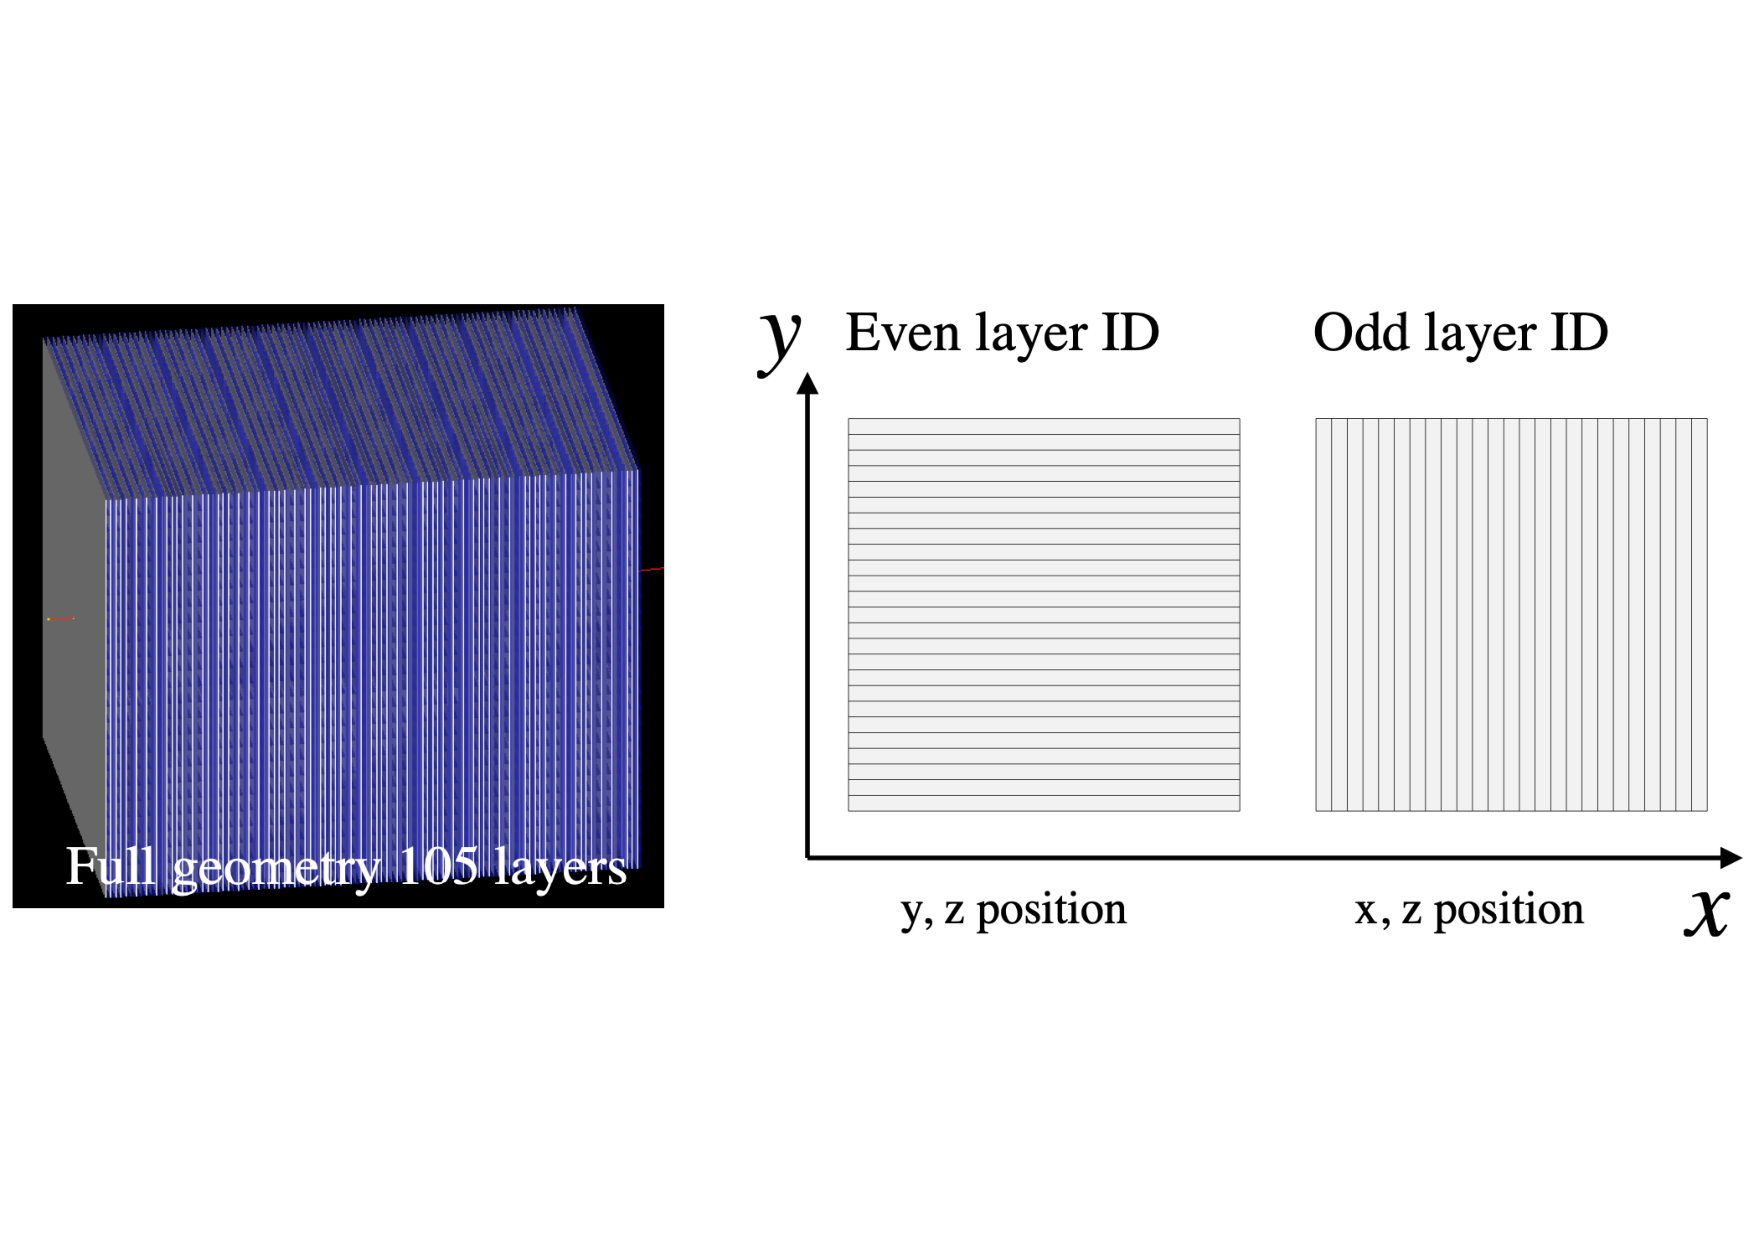
\includegraphics[width=0.85\textwidth]{figures/Sec2/ang_conf.pdf}
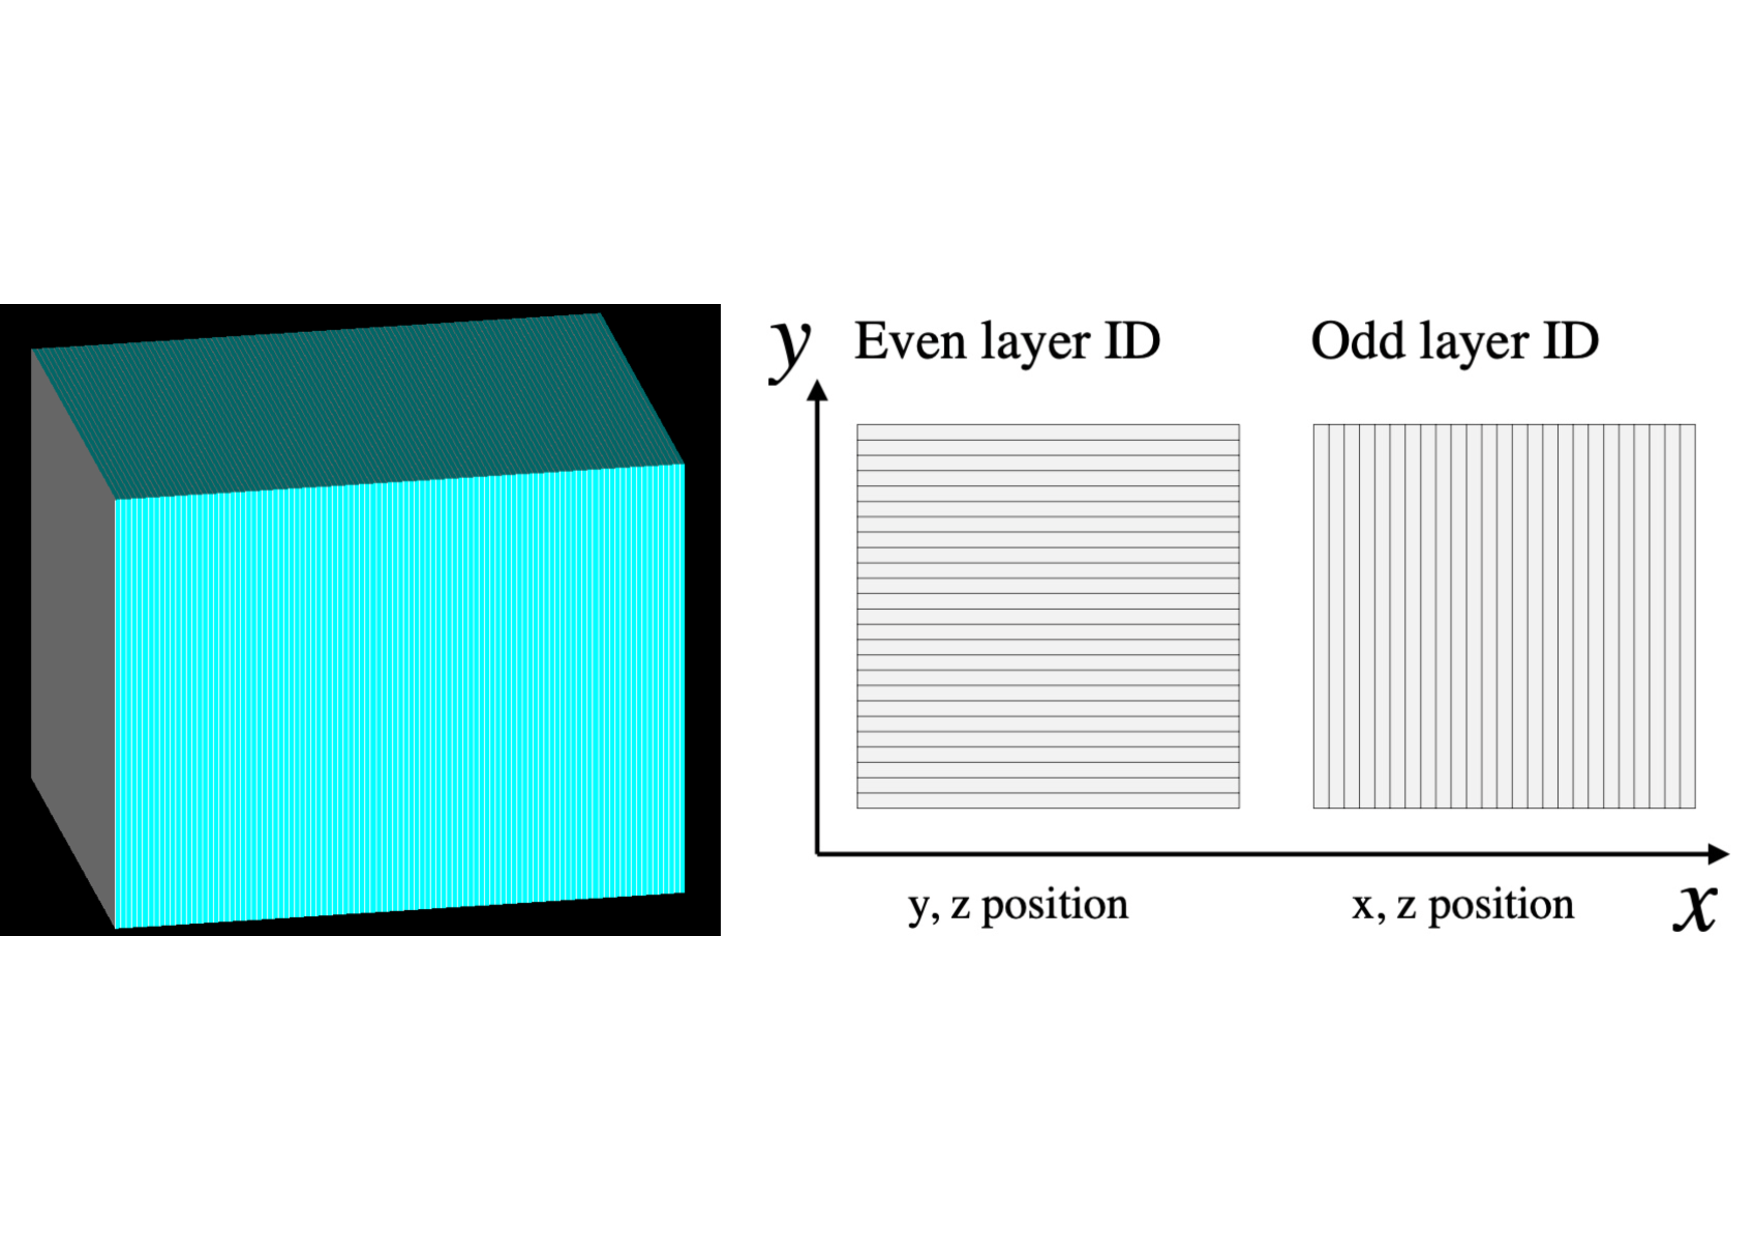
\includegraphics[width=0.85\textwidth]{figures/Sec2/Prototype_samplingcal.pdf}

\caption{ The first trial of detector setup for simulation study on angle measurement. It is a sampling calorimeter consisting of alternating lead sheets and strips of plastic scintillator. }
\label{fig:det_conf}
\end{figure}


%{\it I will describe the coordinator and the gamma enter to the center of strips}
%The contribution of the hadronic interaction is taken into account with $\rm{FTFP\_BERT}$ package. The materials used in detector construction are selected from the Geant4 NIST material database: $\rm{G4\_Pb}$ for the lead and $\rm{G4\_PLASTIC\_SC\_VINYLTOLUENE}$ for the scintillator material.

In order to reconstruct the incident angle of the gamma, we used the $\XGB$, which is one of the popular machine learning packages supporting a scalable tree boosting system~\cite{xgboost:2016}. Input data for the $\XGB$ are deposit energies on each scintillator strip by the generated shower particles. It includes the strips of zero-energy deposit in order to satisfy the requirement that the number of input data should be identical. As the training procedure, the $\XGB$ studies profiles of energy deposit to the individual strips with respect to the incident angle for a given $\gamma$ energy. 

There are five hyper parameters which can be optimized by user, and their values are selected to provide the best angular resolution as described in table~\ref{tab:XgbPar}. Among the parameters, the Max. depth rapidly improves the angular resolution with increasing its value until 15. The N\_estimators also improves the angular resolution with increasing its number, which is correlated to the value of the Max. depth. Its optimal condition becomes 1000 when the Max. depth is 15.

\begin{table}[hbt!]
\centering
\caption{Hyperparameters of the $\XGB$}
\begin{tabular}{cccc}
\hline 
Parameter & Function & Default value & Used value \\ \hline 
N\_estimators & The number of decision trees & N.A. & 1000 \\  
Max. depth & Possible maximum depth of tree structure & 6 & 15 \\ 
Subsample & Fraction of total data used for a single decision & 1 & 1 \\ 
Learning rate & Step length for calculation & 0.3 & 0.08 \\ 
Gamma & Requirement on minimum loss function & 0 & 0 \\ 
\hline
\end{tabular}
\label{tab:XgbPar}
\end{table}

For the training procedure, gammas are generated uniformly in the range 0 to 50 degrees of polar angle ($\theta$) and  0 to 360 degrees of azimuthal angle. The performance of the angular reconstruction is tested with independently generated data samples with fixed $\theta$ and uniform $\varphi$ from 0 to 360 degrees.



%\section{Method}
We started the study with a setup of sampling calorimeter consisting of alternating lead sheet and strips of the plastic scintillator as shown in Fig.~\ref{fig:det_conf}. The electromagnetic shower mainly generated at the lead sheet (passive component) due to its short radiation length ($X_0 = 5.6~{\rm mm})$ and the information of the shower particles is obtained by using the scintillator (active  component). The thickness of lead is 1 mm and scintillator is 5 mm, respectively. The lead sheet has a cross-section of  500 mm $\times$ 500 mm and the scintillator strip of 500 mm $\times$ 15 mm. By arranging the strips in X- and Y-direction alternatively along Z-direction. The generated photon moves along with Z-direction and its incident angle was defined as a polar angle to the direction.  With the configuration, we can get shower profiles in X- and Y-axis in turn, and estimate the incident angle from them. The number of alternating layers is 105, corresponding to 20 radiation length (Xo), in order to contain shower particles fully. 

\begin{figure}[!hbt]
%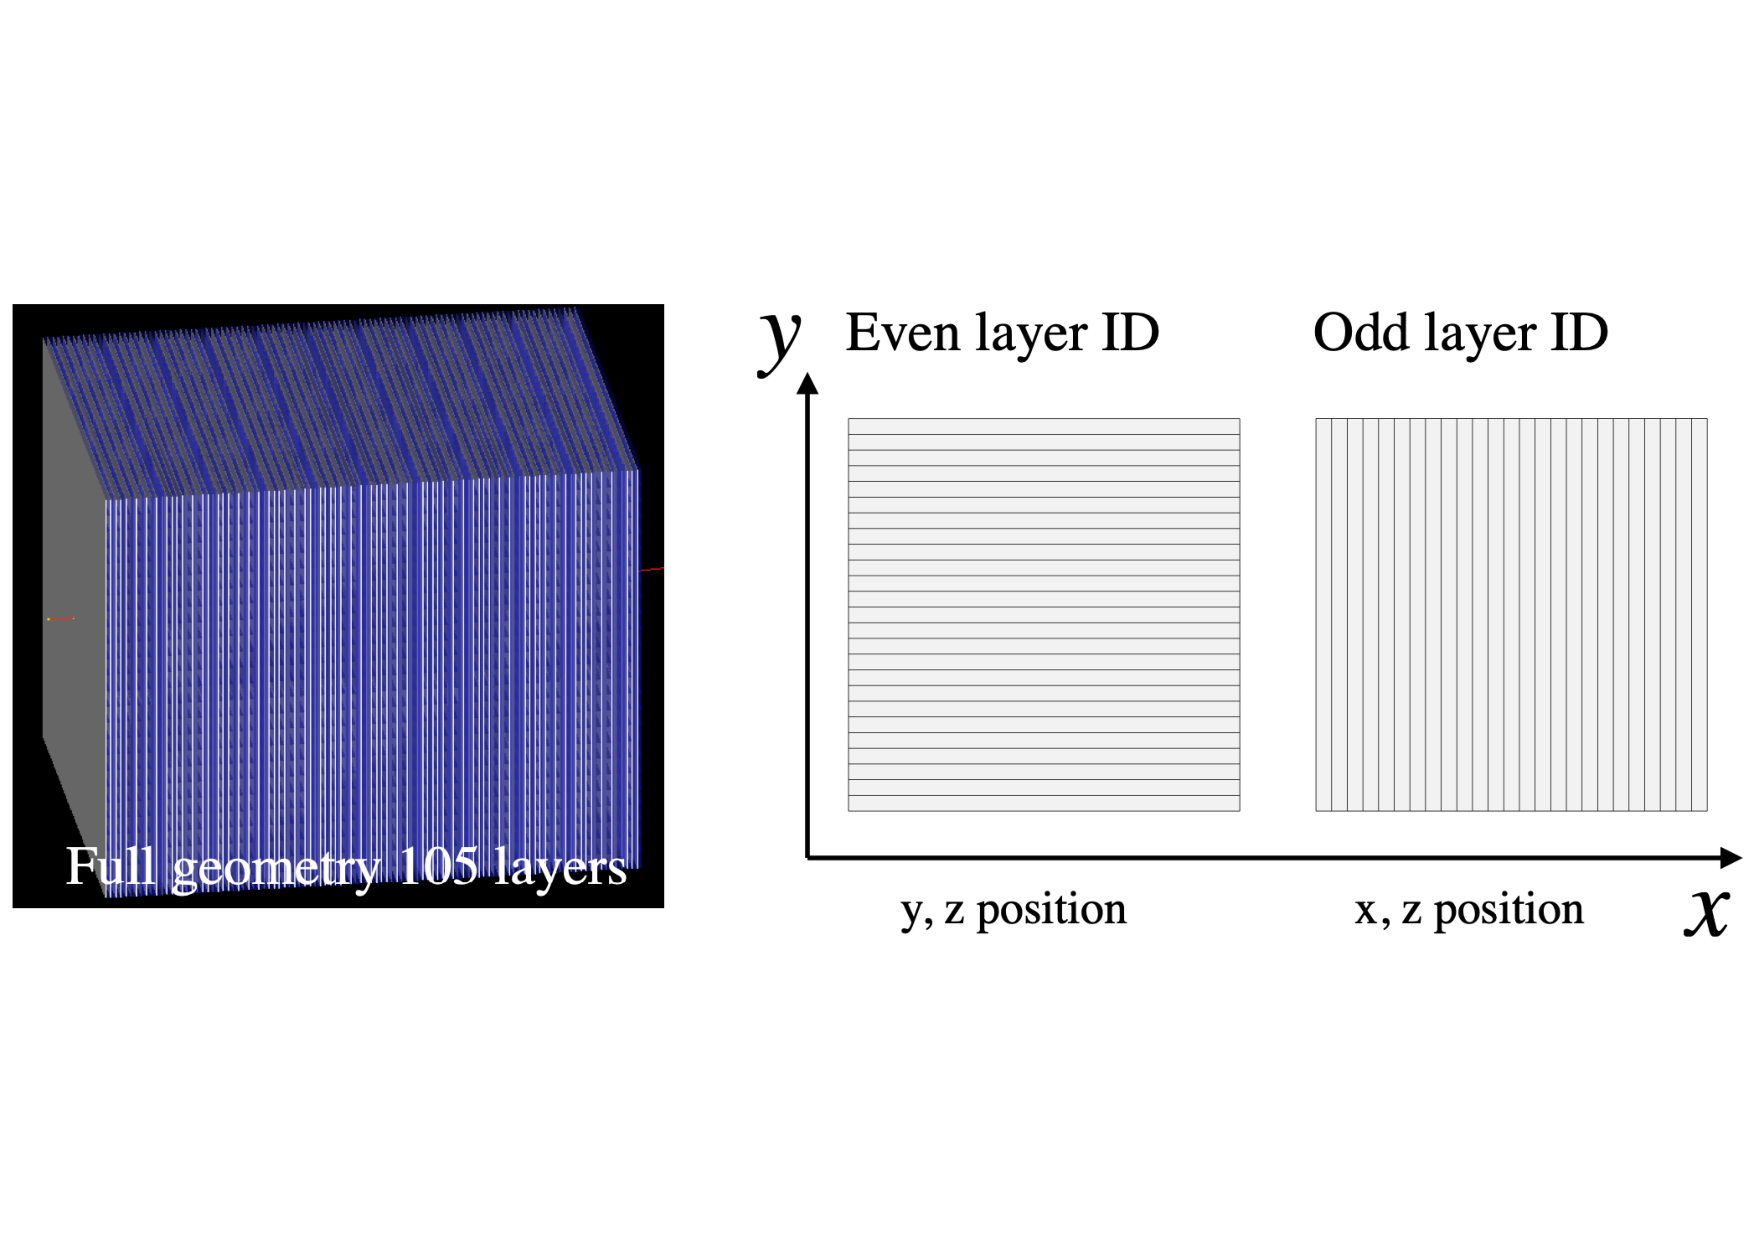
\includegraphics[width=0.85\textwidth]{figures/Sec2/ang_conf.pdf}
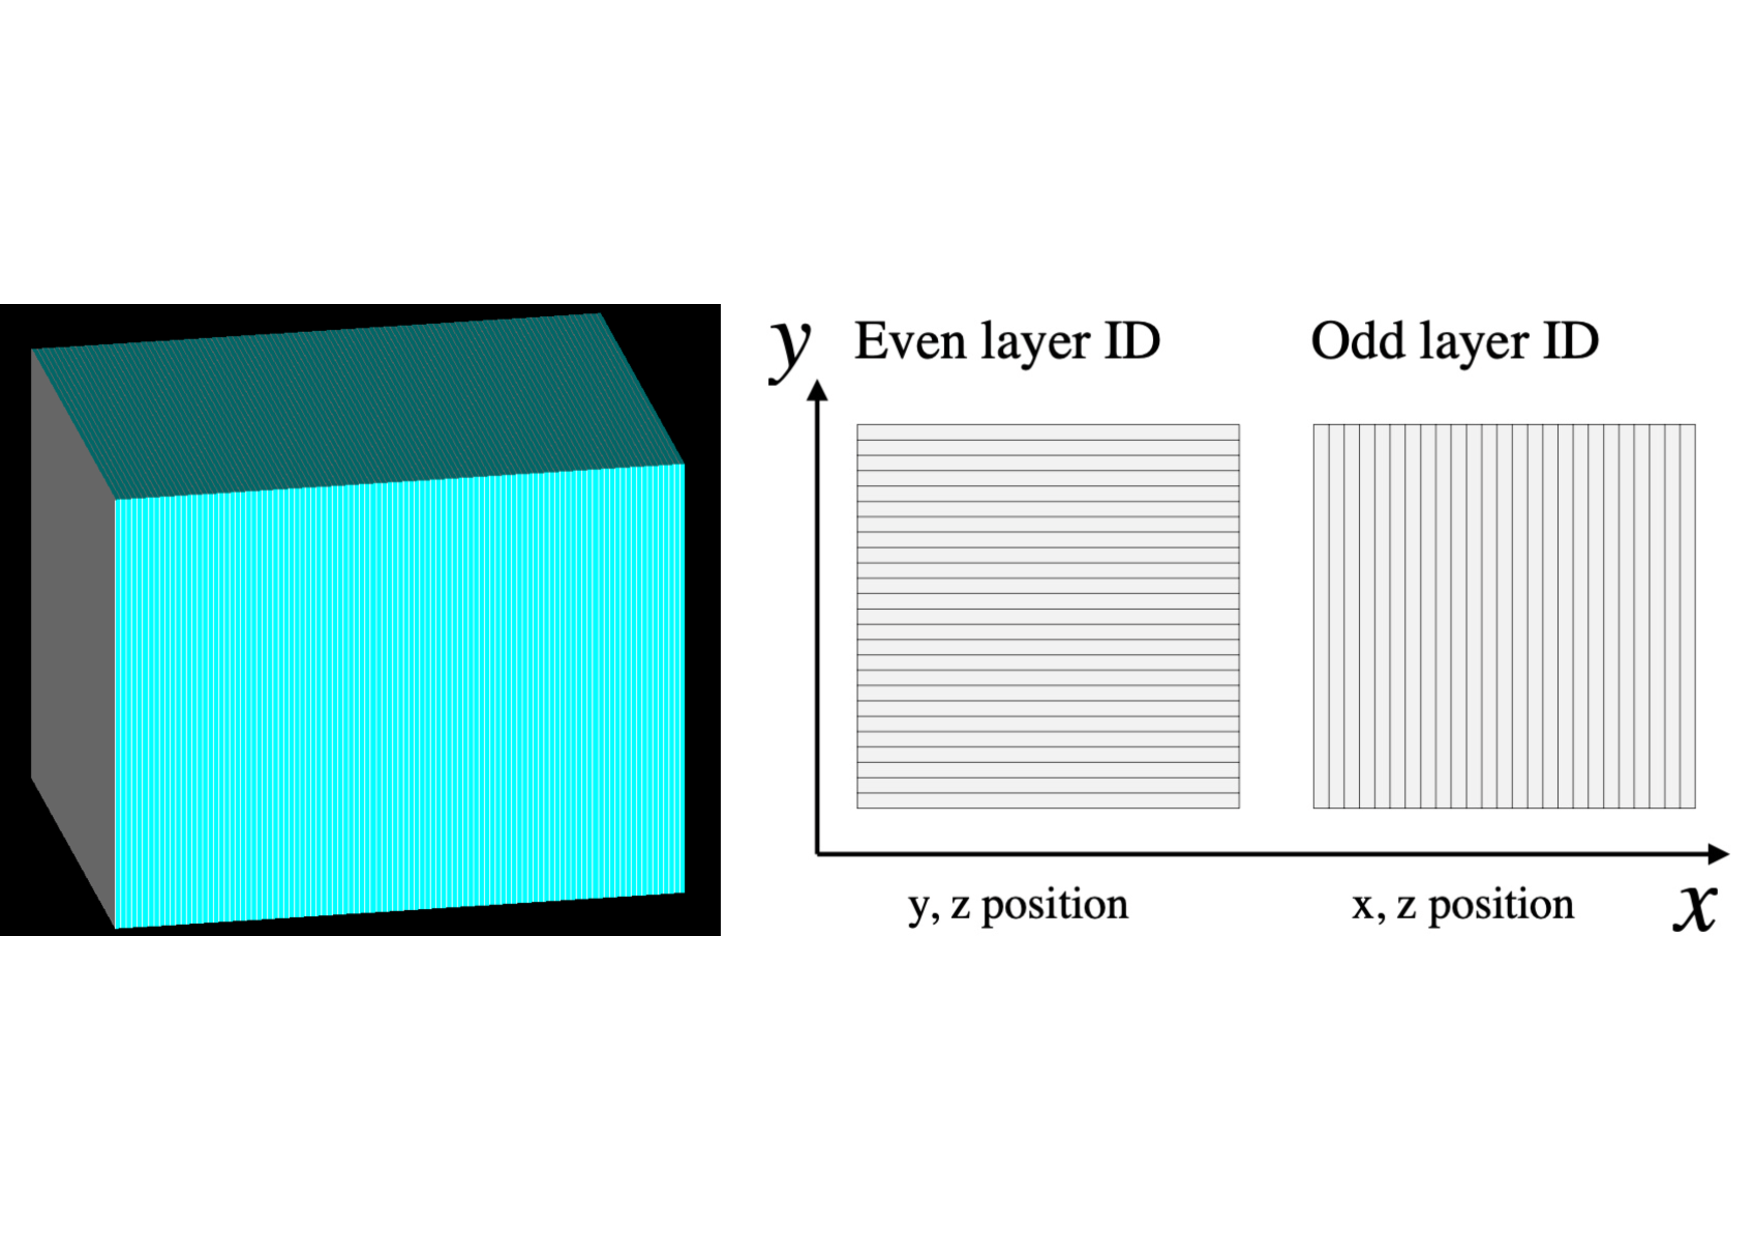
\includegraphics[width=0.85\textwidth]{figures/Sec2/Prototype_samplingcal.pdf}

\caption{ The first trial of detector setup for simulation study on angle measurement. It is a sampling calorimeter consisting of alternating lead sheets and strips of plastic scintillator. }
\label{fig:det_conf}
\end{figure}

The electromagnetic showers are generated with given detector setup by using the GEANT4 package (ver. xxx) with the standard EM sub-packages (URL: https://geant4.web.cern.ch/node/1828). 
${\it I will describe the coordinator}$
%The contribution of the hadronic interaction is taken into account with $\rm{FTFP\_BERT}$ package. The materials used in detector construction are selected from the Geant4 NIST material database: $\rm{G4\_Pb}$ for the lead and $\rm{G4\_PLASTIC\_SC\_VINYLTOLUENE}$ for the scintillator material.

In order to reconstruct the incident angle of the gamma, we used the $\XGB$, which is one of the machine learning packages supporting a scalable tree boosting system~\cite{xgboost:2016}. Input data for the $\XGB$ are deposit energies on each scintillator strip by the generated shower particles. It includes the strips of zero-energy deposit in order to satisfy the requirement that the number of input data should be identical. As the training procedure, the $\XGB$ studies profiles of energy deposit to the individual strips with respect to the incident angle for a given $\gamma$ energy. 

There are five hyperparameters which can be set by user, and their values are selected to provide the better angular resolution as described in tab.~\ref{tab:XgbPar}. Among these hyperparameters, the Max. depth rapidly improves the angular resolution with increasing its value until 100. The N\_estimators also improves the angular resolution with increasing its number up to 1,000 and N\_estimators larger than 1000 does not change the resolution. Its optimal condition becomes 1000 with the Max. depth is 100.

\begin{table}[hbt!]
\centering
\caption{Parameterization of the $\XGB$}
\begin{tabular}{cccc}
\hline 
Parameter & Function & Default value & Used value \\ \hline 
N\_estimators & The number of decision trees & N.A. & 1000 \\  
Max. depth & Possible maximum depth of tree structure & 6 & 100 \\ 
Subsample & Fraction of total data used for a single decision & 1 & 1 \\ 
Learning rate & Step length for calculation & 0.3 & 0.08 \\ 
Gamma & Requirement on minimum loss function & 0 & 0 \\ 
\hline
\end{tabular}
\label{tab:XgbPar}
\end{table}

For the training procedure, gammas are generated uniformly in the range 0 to 50 degrees of polar angle ($\theta$) and  0 to 360 degrees of azimuthal angle ($\varphi$). The performance of the angular reconstruction is tested with independently generated data samples with fixed $\theta$ and uniform $\varphi$ from 0 to 360 degrees.


%\section{method}
%\label{sec:ana}

%\subsection{Geant4 simulation}
%In this paper, the photon shower and corresponding detector responses, the prerequisites for the machine learning inputs, are simulated based on the Geant4 framework. Among several physics packages, the $\rm{FTFP\_BERT}$ physics package is used for electromagnetic and hadronic interactions as it is generally recommended for the high energy physics calorimetry. 

%The materials used in detector construction are selected from the Geant4 NIST material database: $\rm{G4\_Pb}$ for the lead and $\rm{G4\_PLASTIC\_SC\_VINYLTOLUENE}$ for the scintillator material.

%\subsection{Detector construction}
%We constructed a prototype sampling electromagnetic calorimeter with alternative stacking of thin Pb sheets and scintillator strips. A Pb sheet has a dimension of 50 cm (w) $\times$ 50 cm (l) $\times$ 1 mm (t). And a single layer of scintillator plate consists of 25 long scintillator segments, and each segment has a dimension of 2 cm (w) $\times$ 50 cm (l) $\times$ 5 mm (t). The full geometry consists of 105 layers  which is corresponding to 20 $X_0$. In order to investigate the detector properties and test the reconstruction performance of the indicent angle of $\gamma$, we generated $\gamma$ beam data samples with several incident angles and energies.
%In this study, we utilized a physics package $FPFT\_BERT$ for the hadronic and electromagnetic interactions
%We started the study with a setup of sampling calorimeter consisting of alternating lead sheet and strips of plastic scintillator as shown in Fig.~\ref{fig:det_conf}. The thickness of lead is 1 mm and scintillator is 5 mm, respectively. The lead sheet has a cross-section of  500 mm $\times$ 500 mm and the scintillator strip of 500 mm $\times$ 15 mm. By arranging the strips in X- and Y-direction alternatively along Z-direction. The generated photon moves along with Z-direction and its incident angle was defined as a polar angle to the direction.  With the configuration, we can get shower profiles in X-Z and Y-Z planes in turn, and estimate the incident angle from them. The number of alternating layers is 105, corresponding to 20 radiation length (Xo), in order to contain shower particles fully. 

%\begin{figure}[!hbt]
%%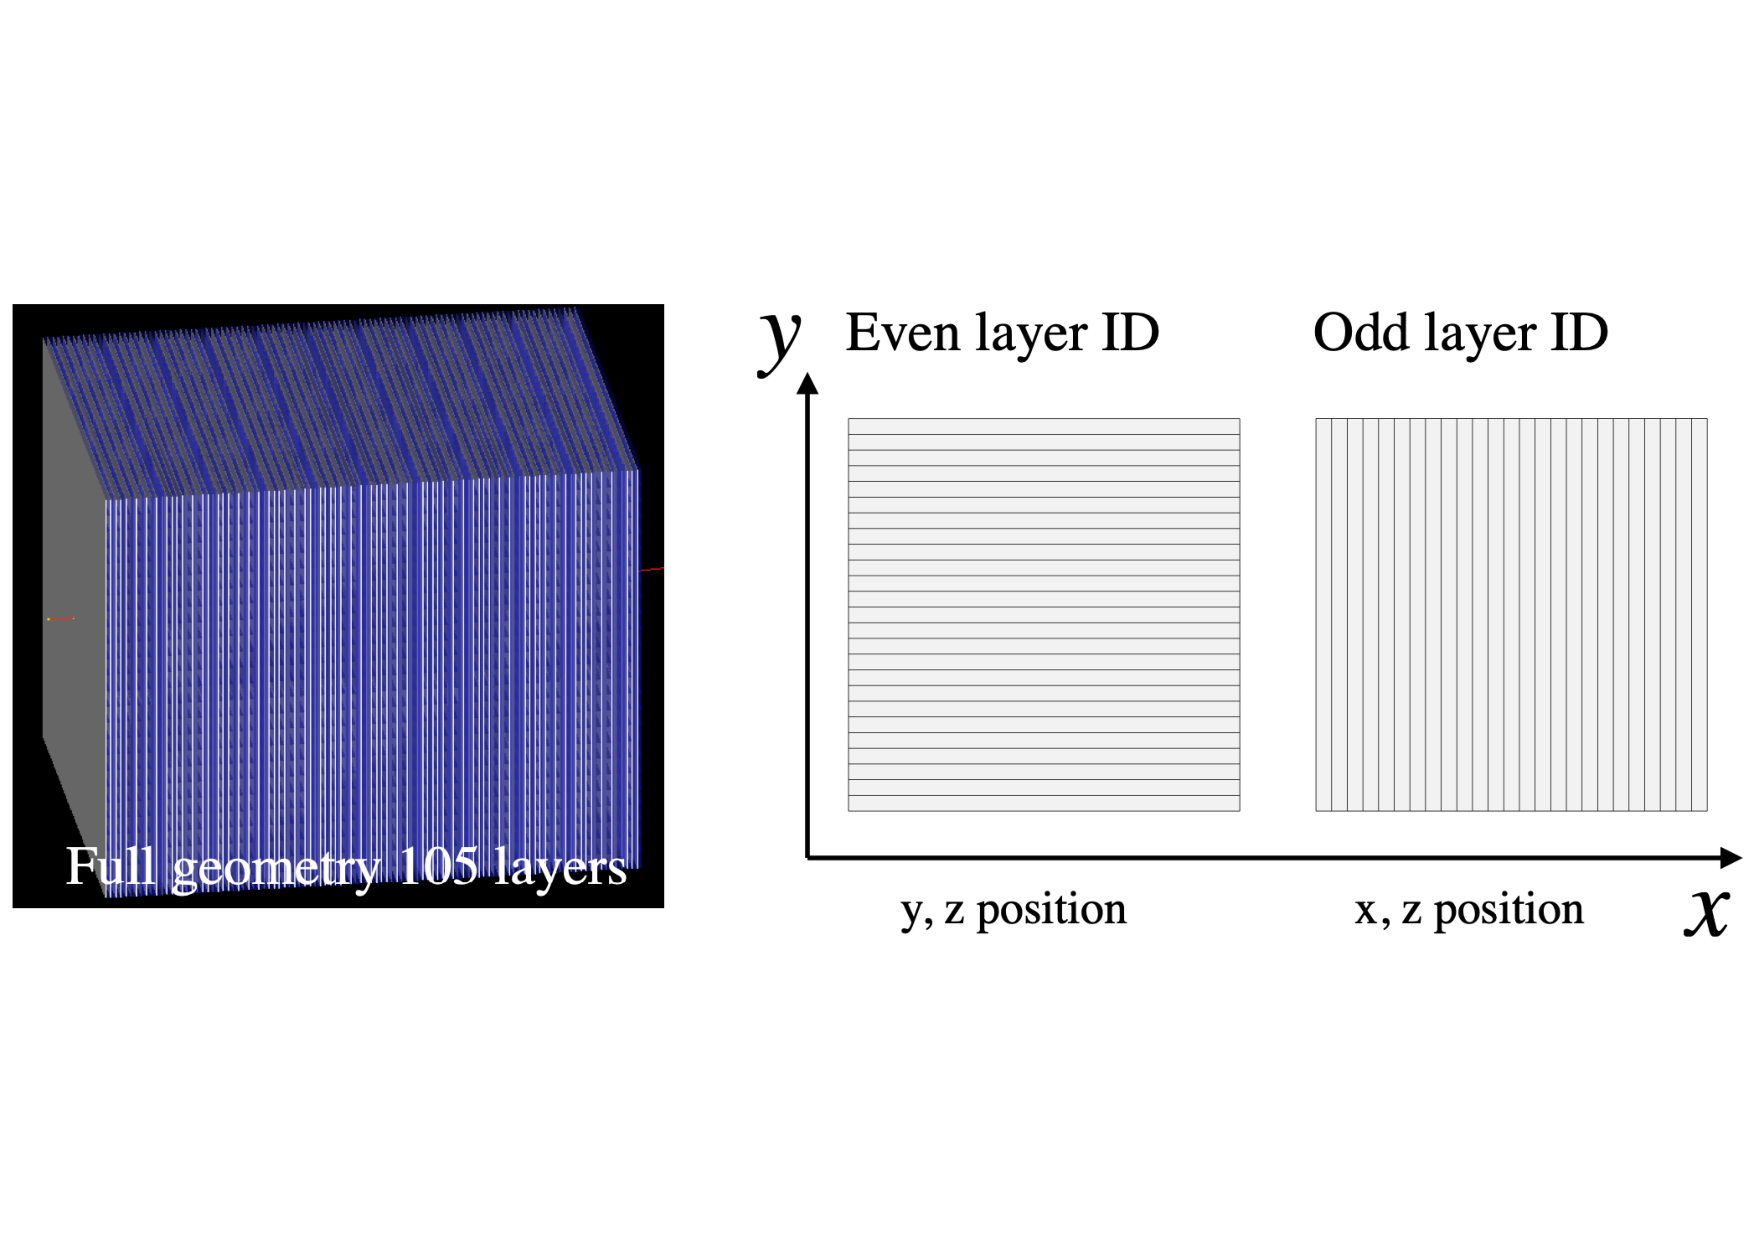
\includegraphics[width=0.85\textwidth]{figures/Sec2/ang_conf.pdf}
%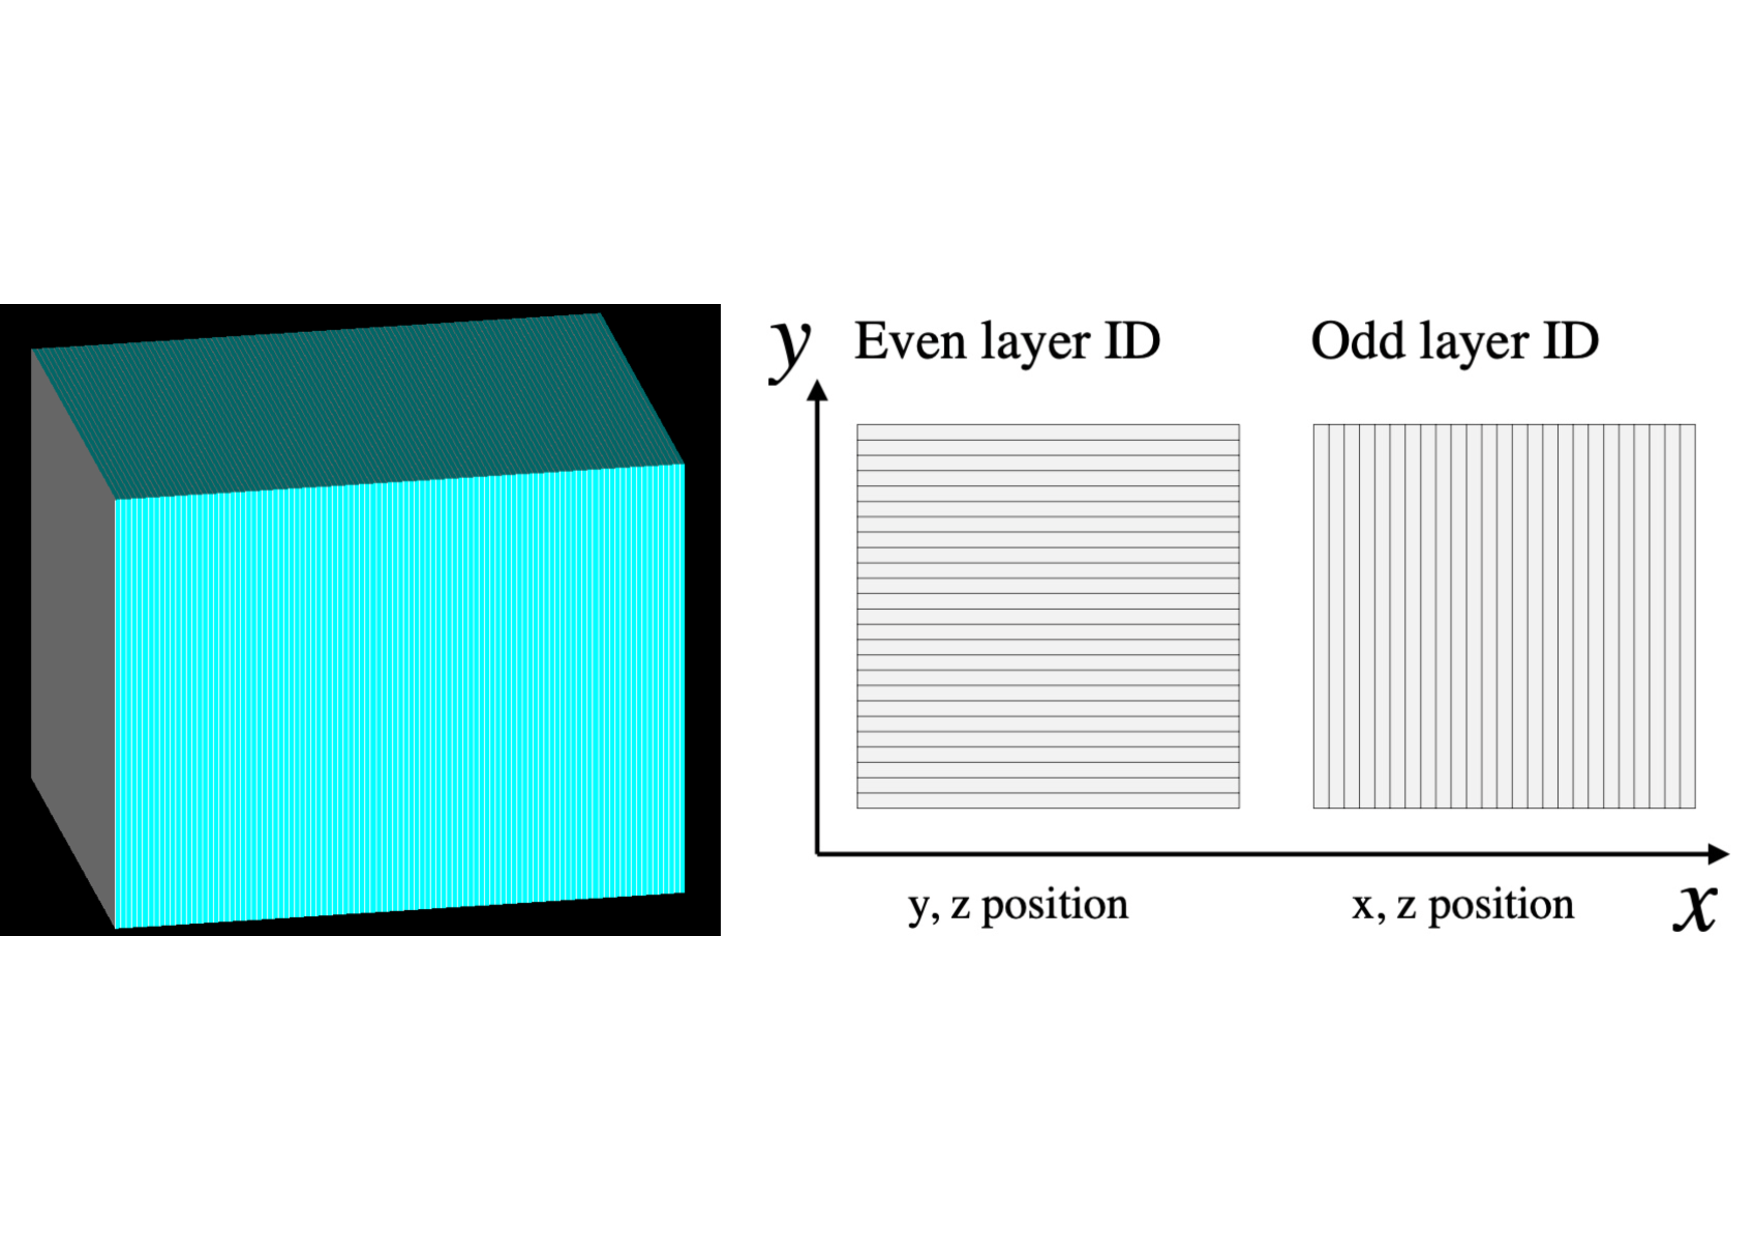
\includegraphics[width=0.85\textwidth]{figures/Sec2/Prototype_samplingcal.pdf}

%\caption{ The first trial of detector setup for simulation study on angle measurement. It is a sampling calorimeter consisting of alternating lead sheets and strips of plastic scintillator. }
%\label{fig:det_conf}
%\end{figure}

%\subsection{Electromagnetic shower Generation}
%\subsection{Properties of electromagnetic shower (EM shower)}
%We generated the EM shower generated inside the detector with GEANT4, which provides reliable results for them polish-up later).


%\subsection{Properties of electromagnetic shower (EM shower)}

%In general, the less the photon shower develops in the transverse direction, the more separable the photon clusters, and the higher the visible ratio, the better the energy resolution. However, these properties are incompatible as they have strong inverse correlation. For the trade-off configuration, we investigated the Molière radius and the visible ratio with several configurations. 

% 어떤 configuration, energy? 등등
% 2.5, 5, 10, 15, 20 mm for scint., 0.5, 1, 2 mm for lead 1GeV gamma
% For energy resolution, 100 MeV step 100MeV ~ 2GeV gamma


%\subsection{Backsplash}
% backsplash particle이 veto signal을 만들어 accidental event loss를 만든다.
% incident photon의 에너지와 각도를 바꿔가며 front surface로 빠져나오는 backsplash particle의 개수를 카운팅
% 1개 이상의 backsplash particle이 있으면 veto에 counting

%\subsection{XGBOOST: A toolkit for machine learning}
%\label{sec:anaML}
%Among many packages for machine learning in the high energy physics area~\cite{ATLAS:2020iwa}, we used the $\XGB$, supporting a scalable tree boosting system~\cite{xgboost:2016}. The $\XGB$ package is used to reconstruct the incident angle of incident $\gamma$ particles with deposit energies in the each channel, where secondary particles of the EM shower raise signals. Input data for the $\XGB$ are deposit energies for whole channels including zero-energies to tally with the requirement that the number of input data should be identical. For the $\XGB$ to reconstruct the angle, the training procedure for the $\XGB$ needs to be preceded. The training procedure helps the $\XGB$ study how $\gamma$ interacts with the detector and deposits the energy to the each channel with respect to the incident angle for a given $\gamma$ energy. Simulations are done with the uniform incident polar angle ($\theta$) distribution from 0 to 50 degree and the uniform azimuthal angle ($\varphi$) from 0 to 360 degree for the training, which makes the $\XGB$ possible to reconstruct events having 0~$<\theta<$~50~degree and 0~$<\varphi<$~360~degree. The reconstruction of $\theta$ by the $\XGB$, completing the training procedure, is tested with the fixed $\theta$ and uniform $\varphi$ from 0 to 360 degree.

\section{Results}
\label{sec:res}


\subsection{Properties of generated shower}
% moliere rad, visible ratio graph
% energy resolution (+as a function of E)
% gamma beam energy에 따라 backsplash가 만드는 event veto
% + incident angle에 따라?
Figure \ref{fig:EMshower} shows shower profiles in X-Z plane (right) and Y-Z plane (middle), those are accumulated energy deposit on each strips for 10,000 gammas of energy as 1 GeV.
%longitudinal (right) and lateral (left) shower development for 1 GeV photon entering perpendicular to the detector surface $(\theta~=0)$). 
Its longitudinal projection (left in Fig.\ref{fig:EMshower}) %roduced by gamma of energy as $E_0$ 
can be expressed by two parameters $\alpha$ and $\beta$ as %{ref:E. Longo, I. Sestili, Nucl. Instrum. Meth. 128 (1975) 283 }
\begin{equation}
    F(E,t)=E_0\cdot (bt)^{a-1}e^{-bt}/\Gamma(a),
    %F(E,t)=E_0\cdot t^{\alpha}e^{-\beta t},
\end{equation}
where t is the z-position in radiation length. It is natural that the distributions on converter and counter are identical. 
%When we consider detector response for large number of gamma, it is needed another contribution $t_0$ which is the starting position of shower generation. Then the equation 1 becomes as
%\begin{equation}
    %F(E,t)=E_0\cdot b(bt)^{a-1}e^{-bt}/\Gamma(a),
%    F(E,t,t_0)=E_0\cdot e^{-t_0 / X_0} (t-t_0)^{\alpha}e^{-\beta (t-t_0)},
%\end{equation}
%or
%\begin{equation}
    %F(E,t)=E_0\cdot b(bt)^{a-1}e^{-bt}/\Gamma(a),
%    F(E,t)= \integral { E_0\cdot e^{-t_0 / X_0} (t-t_0)^{\alpha}e^{-\beta (t-t_0)}},
%\end{equation}
%The parameters are estimated for given detector with 1 GeV $\gamma$ as a= and b=, respectively.

On the other hand, the transverse shower spread is interpreted as a distribution of energy deposit in crossing positions of the X- and the Y-strips in neighbouring two layers as shown in Figure XXX.  This distribution is expressed by the Molière radius defined as 
\begin{equation}
\rho_M= 21.2~{\rm MeV}\cdot X_0 /E_c,
\end{equation}
where $X_0$ is the radiation length and $E_c$ is the critical energy of the detector, respectively. 
For the sampling calorimeter consisting of different materials, let us define the Molière radius as the radius of cylinder containing 90\% of shower energy. As shown in Figure xxx, the test model (1-mm lead and 5-mm scintillator) shows $\rho_M=70$ mm in average which changes with the shower depth. 
That is, we can expect an improvement on separating two gammas closely incident to the calorimeter. We will study on this subject and not treat in this paper.
%the For the detector consisting of 1mm lead and 5mm plastic scintillator contain 90\% of energy deposit inside the cylinder of radius of $\rho_M=70$ mm. %It had better to compare with CsI crystal

The energy resolution of the sampling calorimeter is mainly determined by the fluctuation of the visible ratio defined as 
\begin{equation}
R = { \frac{E_{act}} {E_{act}+E_{pas}}},
\end{equation}
where $E_{act}$ and $E_{pas}$ are energy deposit to the active and passive part of the calorimeter, respectively. This visible ratio is roughly given by a ratio of material budget between the converter and the counter. 
%is simply given by the fraction of the active component to that of the passive component, and its fluctuation becomes large when the ratio is small.
%by thickness of the converter. It is because the energy deposit at the active component is done through not only passage of the electron-positron pair but also low energy process such as compton scattering not reach to the active counter. 
As shown in Fig.~\ref{fig:energy_res}, the mean of the visible ratio for the configuration of 1-mm lead and 5-mm scintillator is  0.35 and its energy resolution is expected 4\% for 1 GeV photon. However, the visible ratio can be improved with the same amount of composed materials when we use thinner layers. Figure YYY shows the change of the visible ratio for the same ratio $R=t_{lead}/t_{scin}$=0.2 according to the thickness of the converter (thinner scintillator too). When we make the lead sheet thinner as a factor of 5, the visible ratio improves as XXX. This is because the number of low energy electrons and positrons penetrating the lead sheet. Even though the small improvement on the visible ratio, the energy resolution improved greatly with the thinner layer.
%This energy resolution is improved as a result thinner converter and counter keeping the visible ratio constant.


\begin{figure}[!hbt]
%\includegraphics[width=0.85\textwidth]{figures/Sec2/EMshower.pdf}
%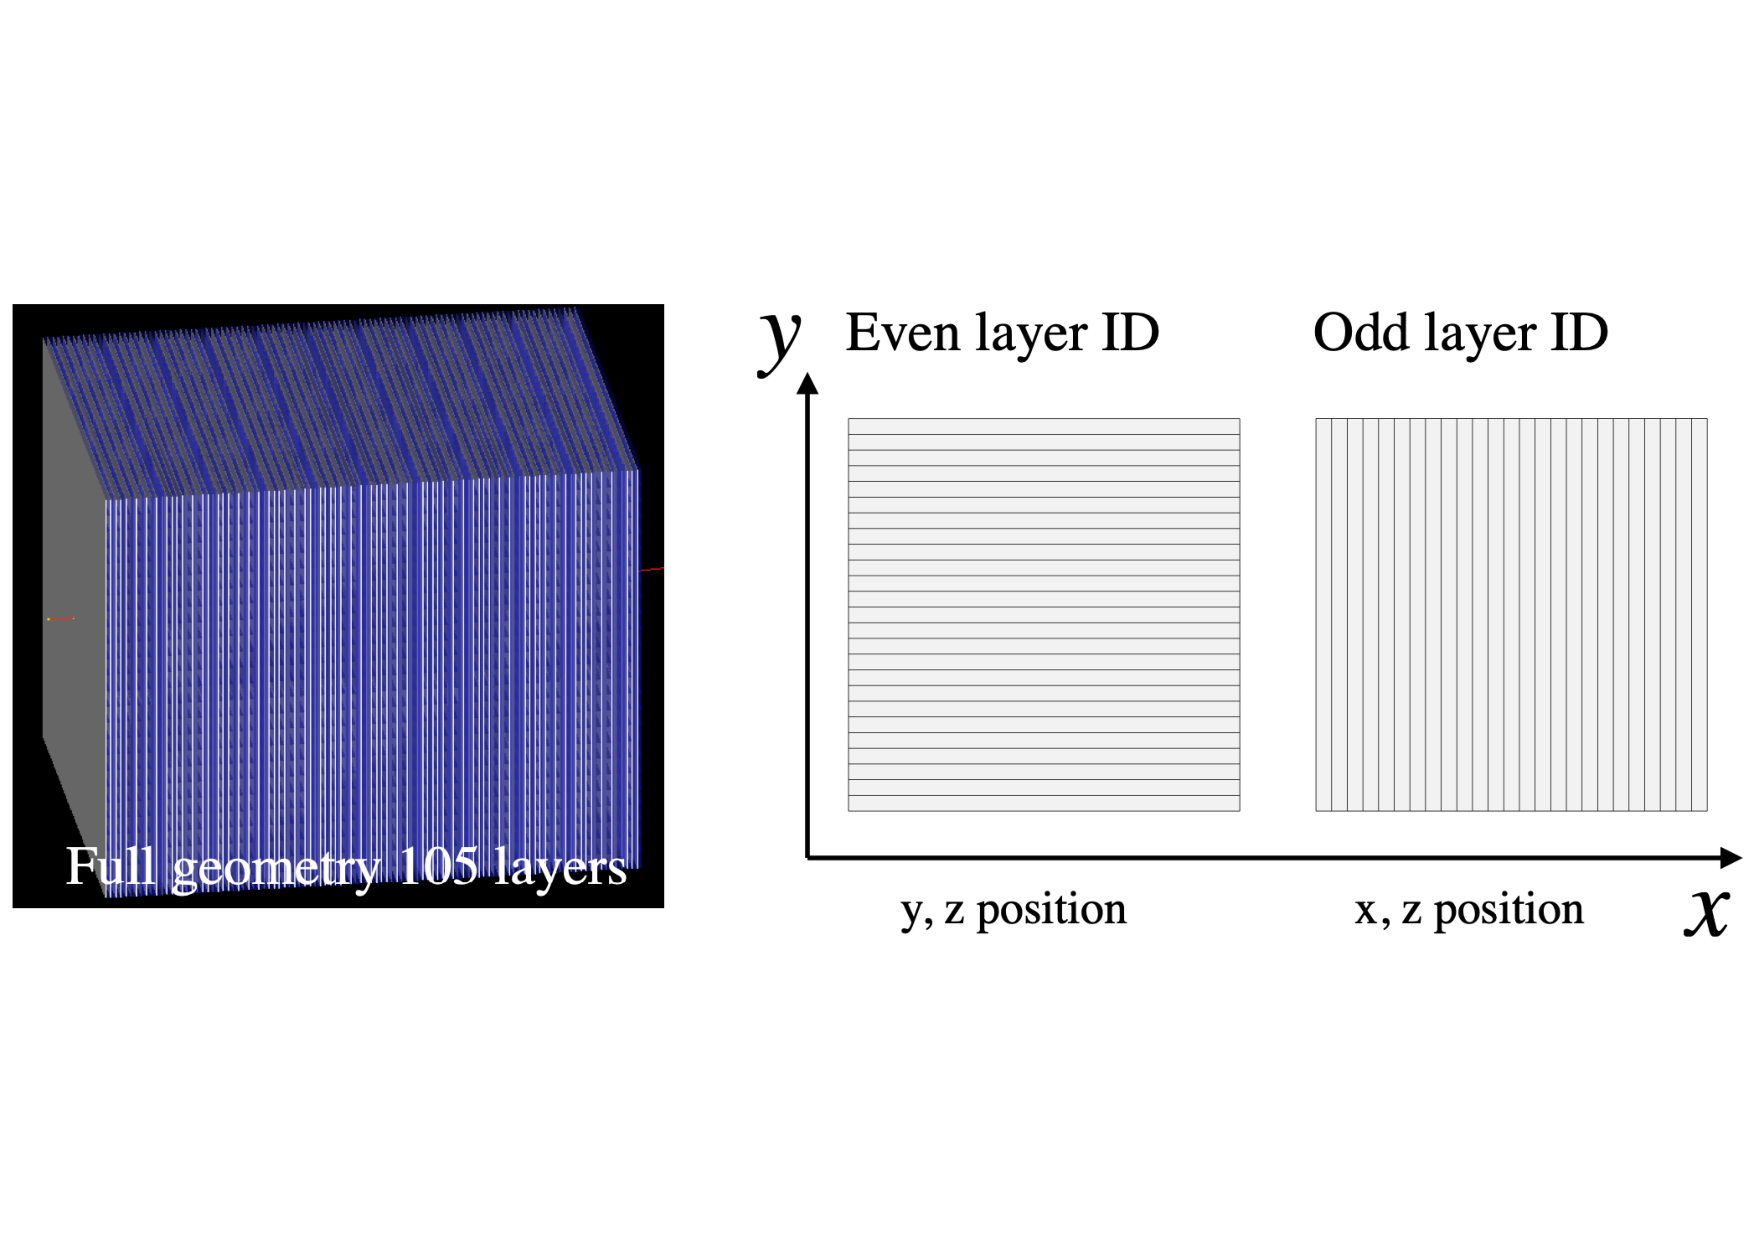
\includegraphics[width=0.85\textwidth]{figures/Sec2/ang_conf.pdf}
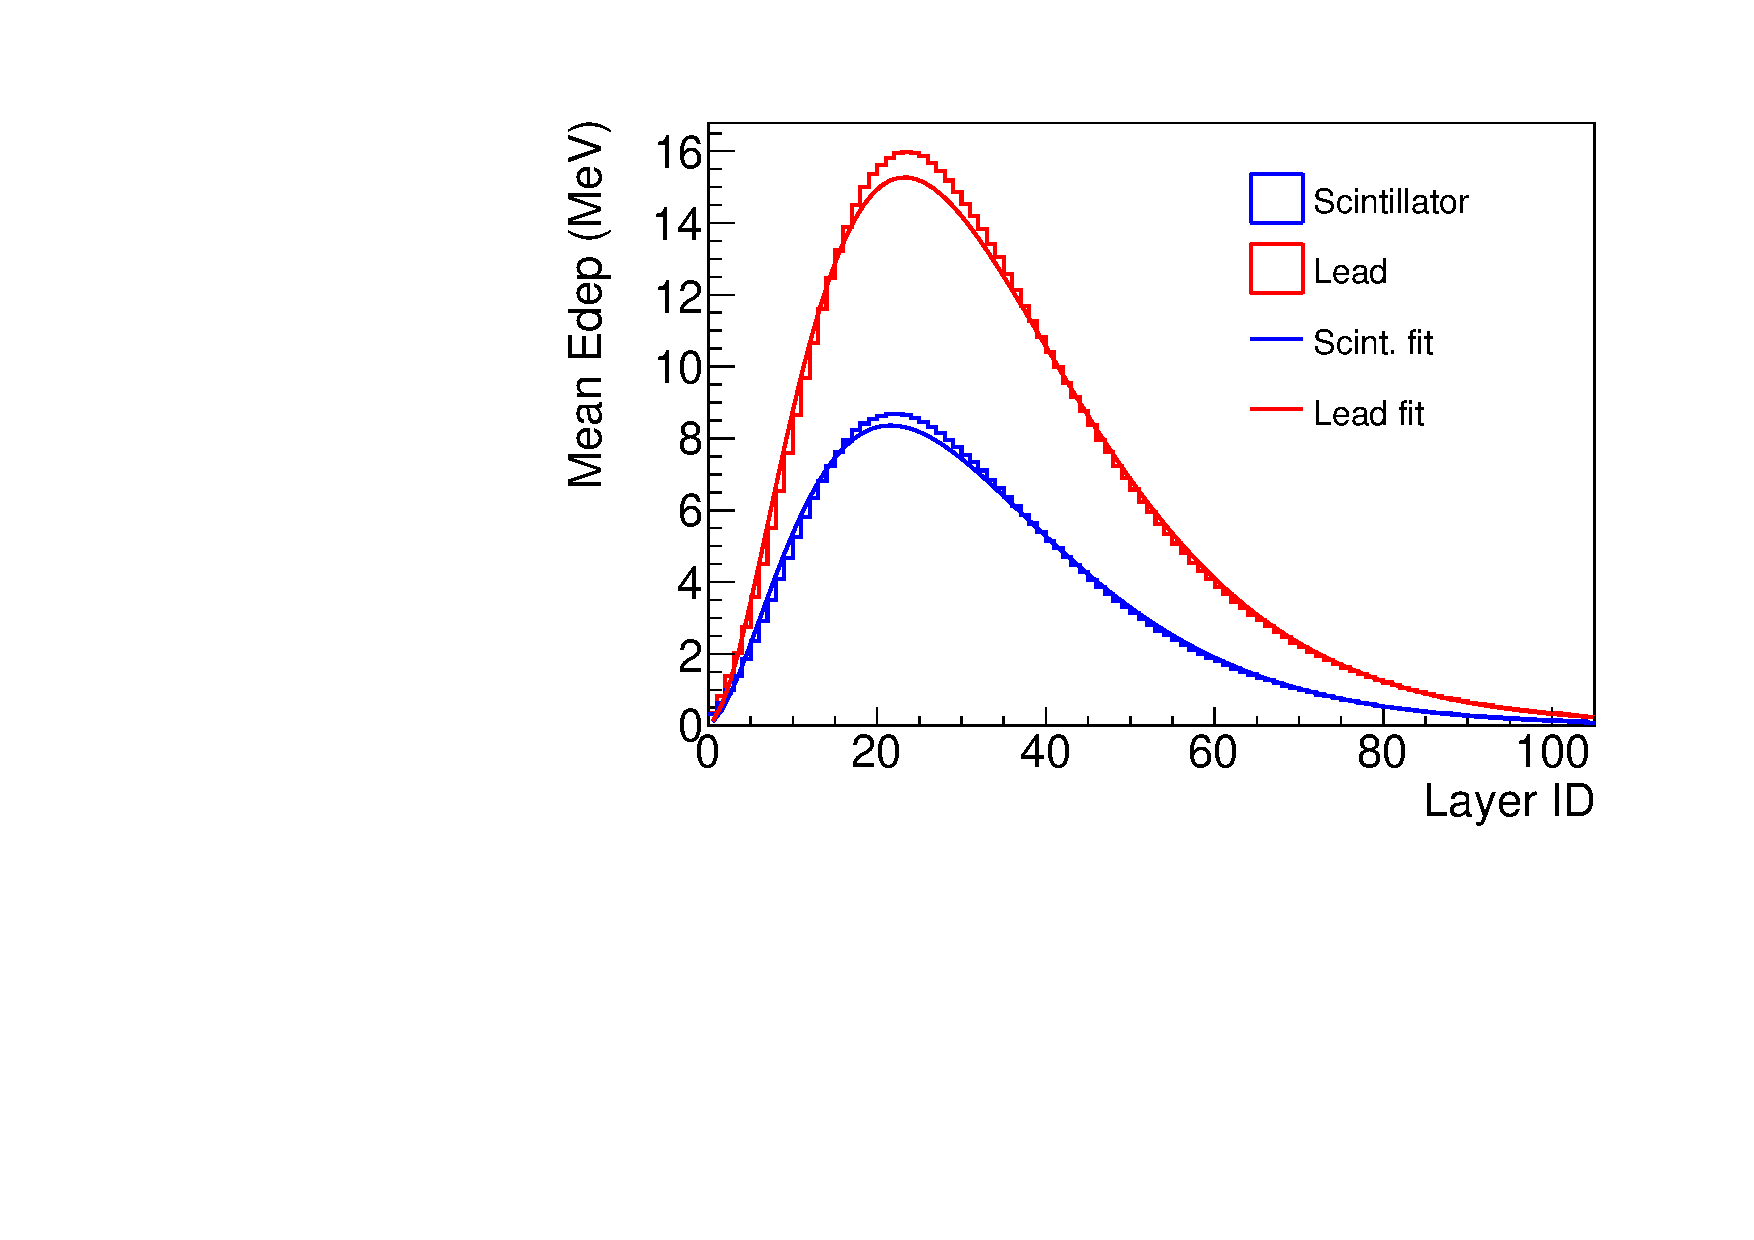
\includegraphics[width=0.48\textwidth]{figures/Sec2/ShowerProfileZ.pdf}
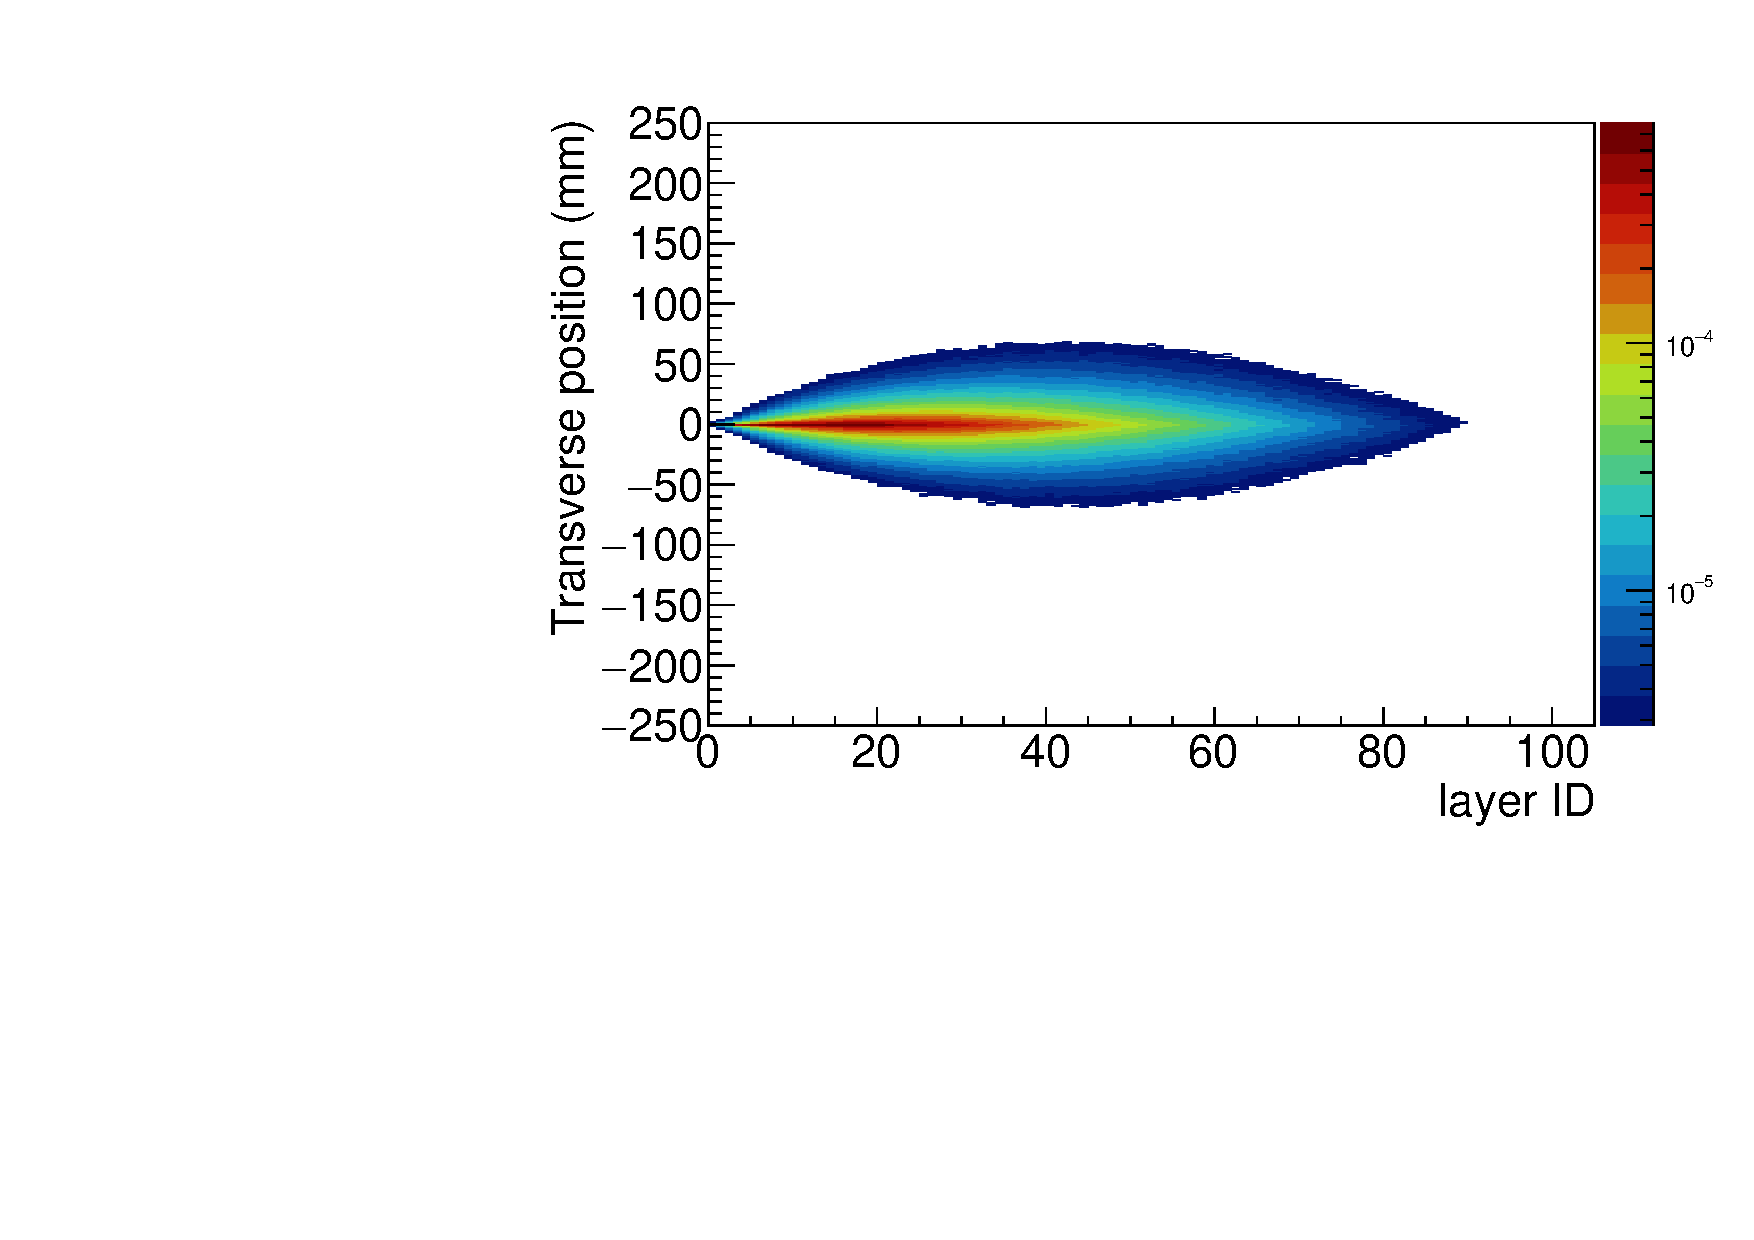
\includegraphics[width=0.48\textwidth]{figures/Sec2/ShowerProfileXZ.pdf}
\caption{Profile of the EM shower in Z axis(left) and X-Z plane(right)  }
\label{fig:EMshower}
\end{figure}


\begin{figure}[!hbt]
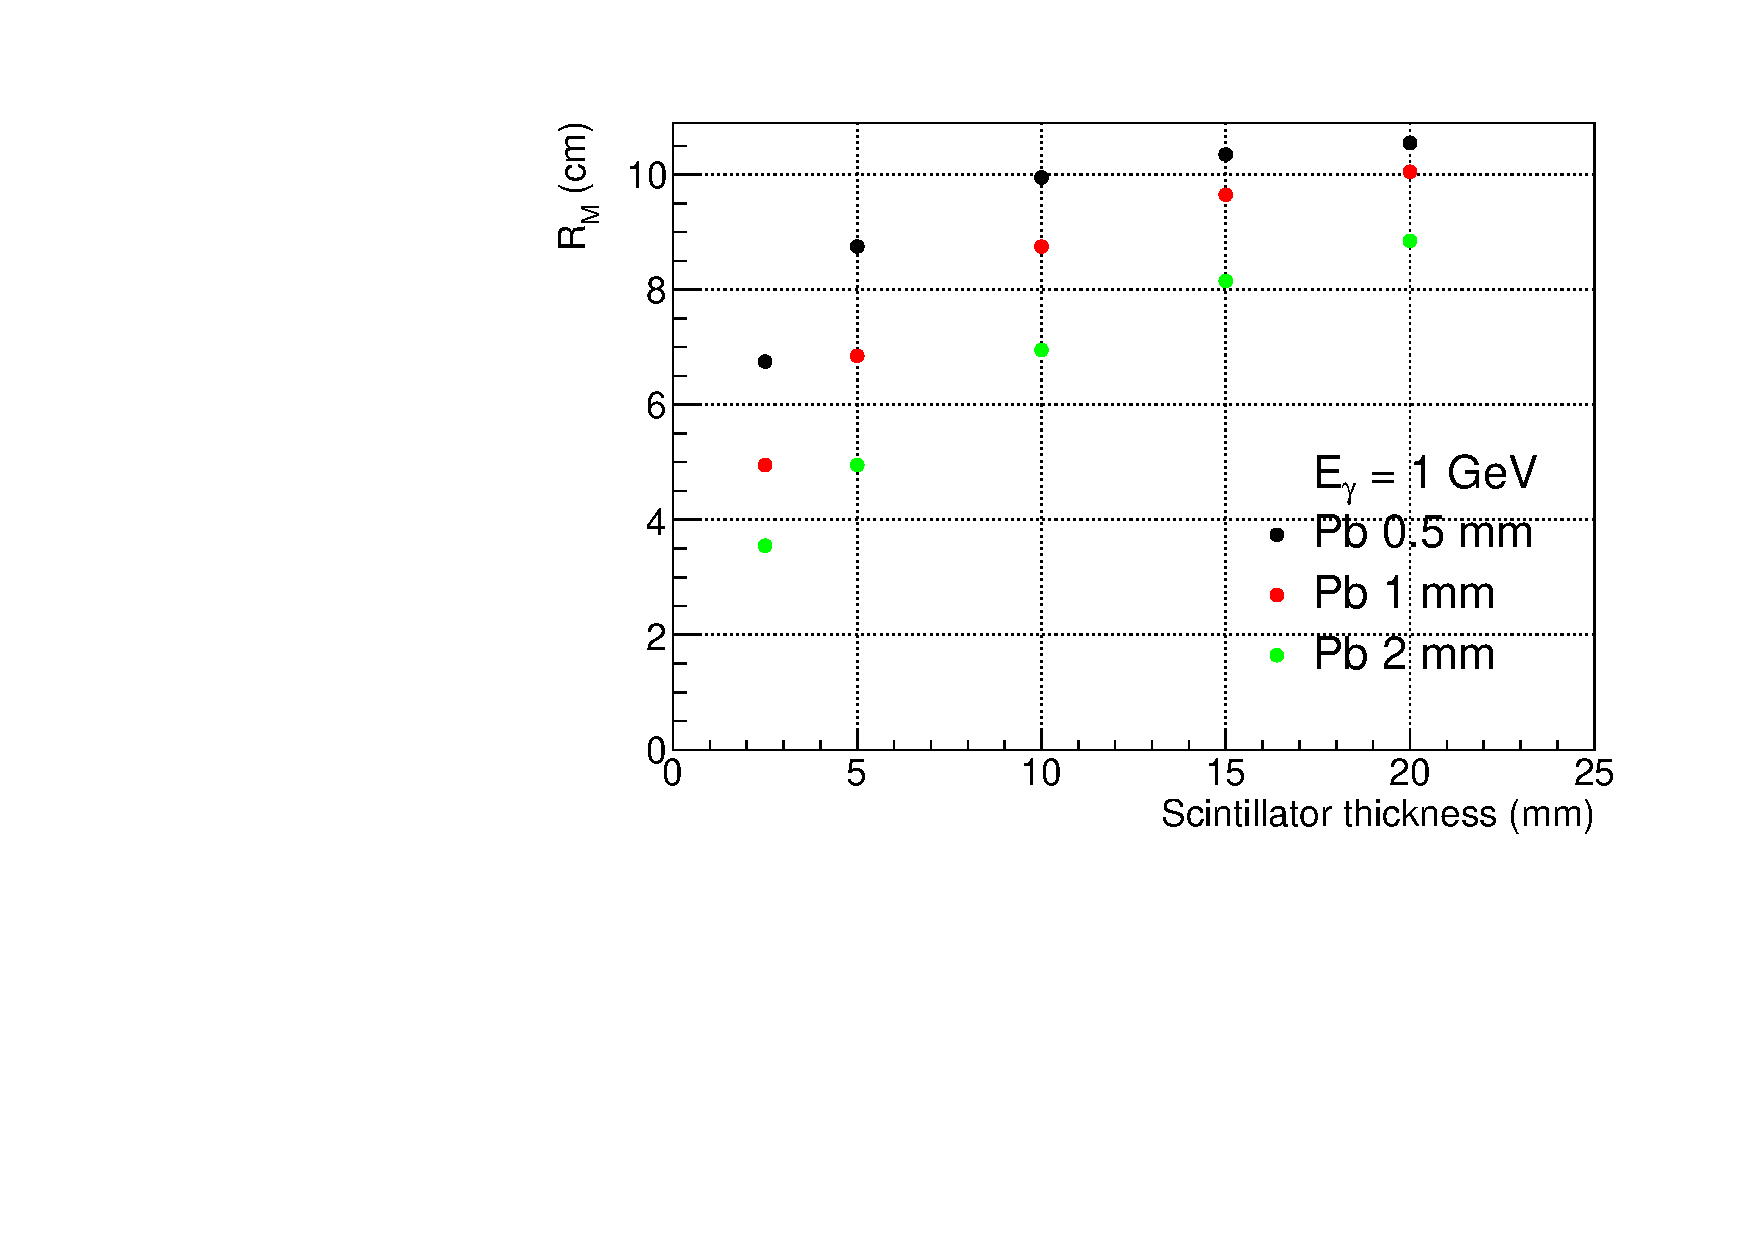
\includegraphics[width=0.48\textwidth]{figures/3.2/moliere_radius.pdf}
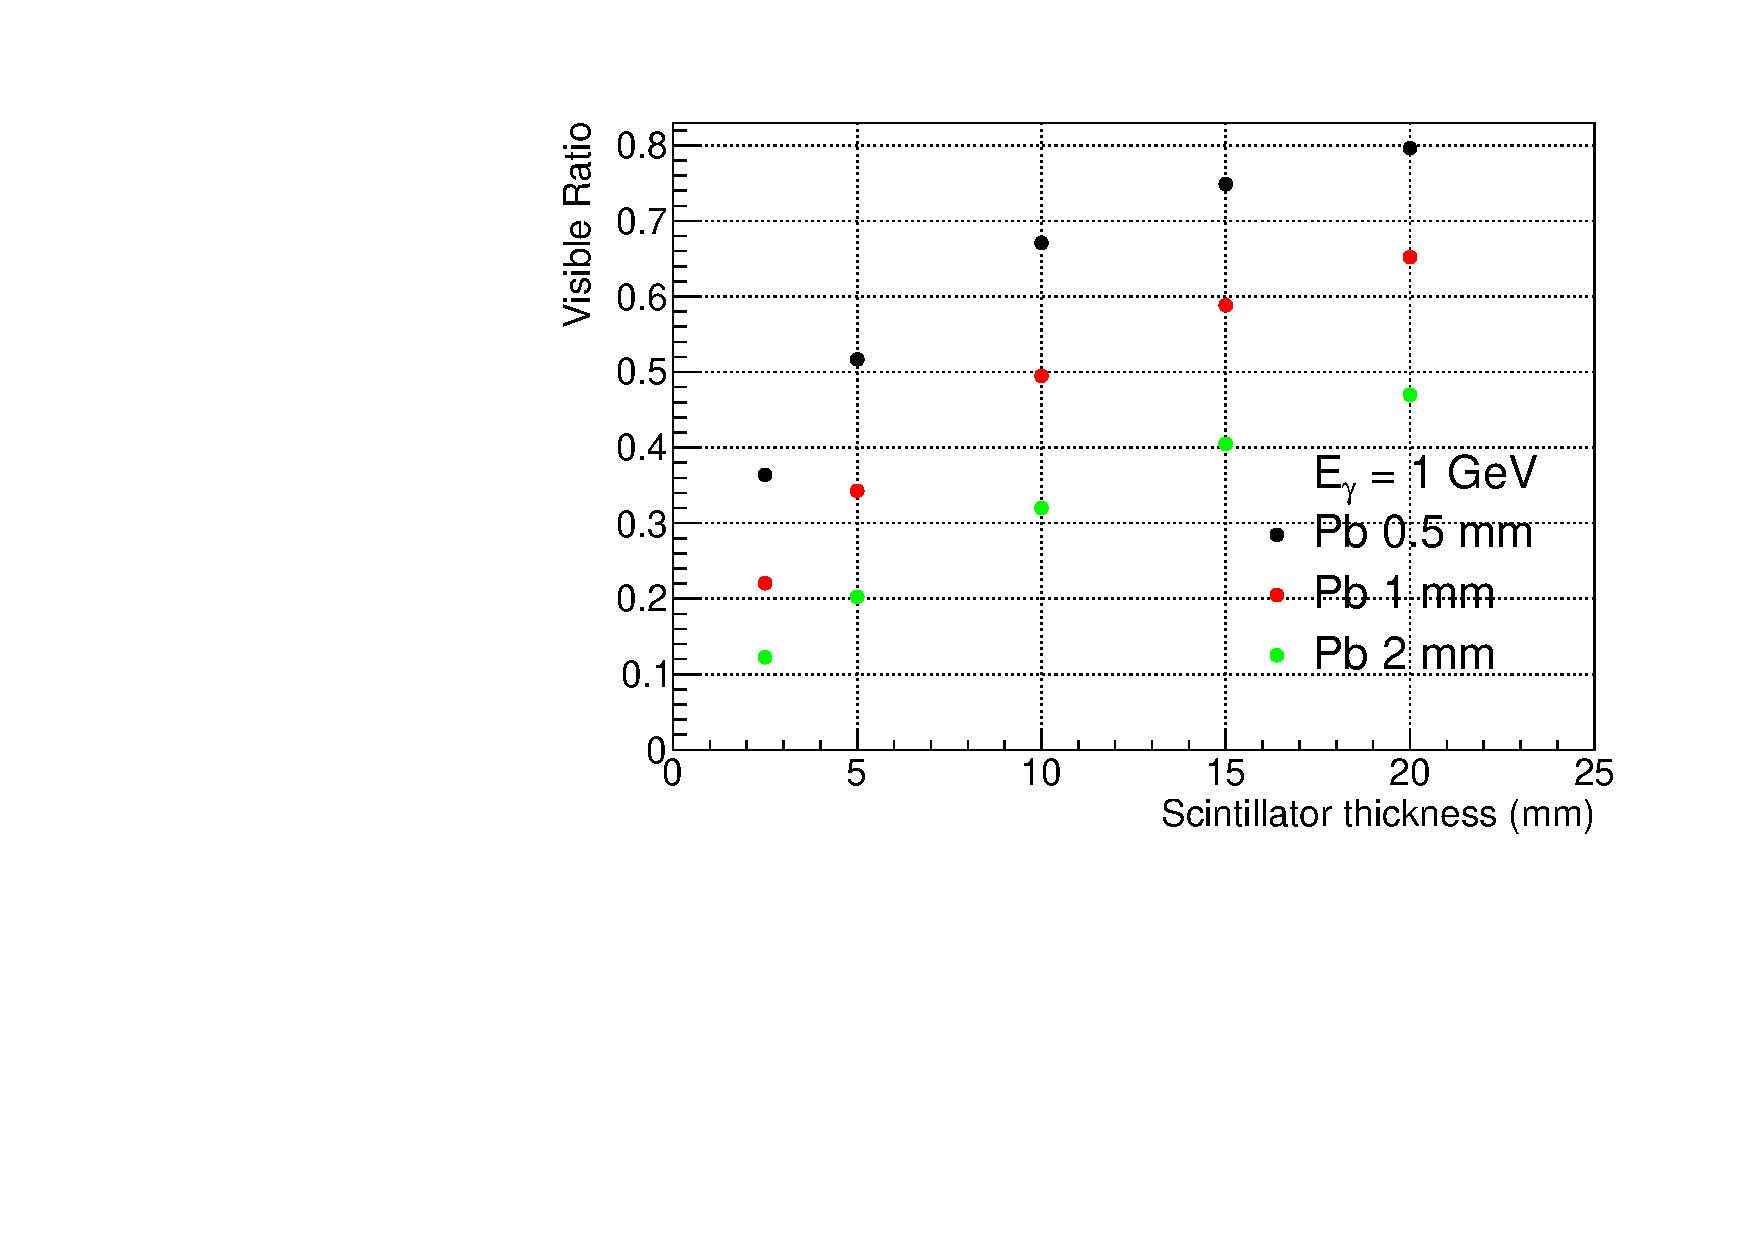
\includegraphics[width=0.48\textwidth]{figures/3.2/visible_ratio.pdf}
\caption{Dependence of Moliere radius(left) and visible ratio(right) on the thickness of scintillators}
\label{fig:moliere_vis}
\end{figure}

\begin{figure}[!hbt]
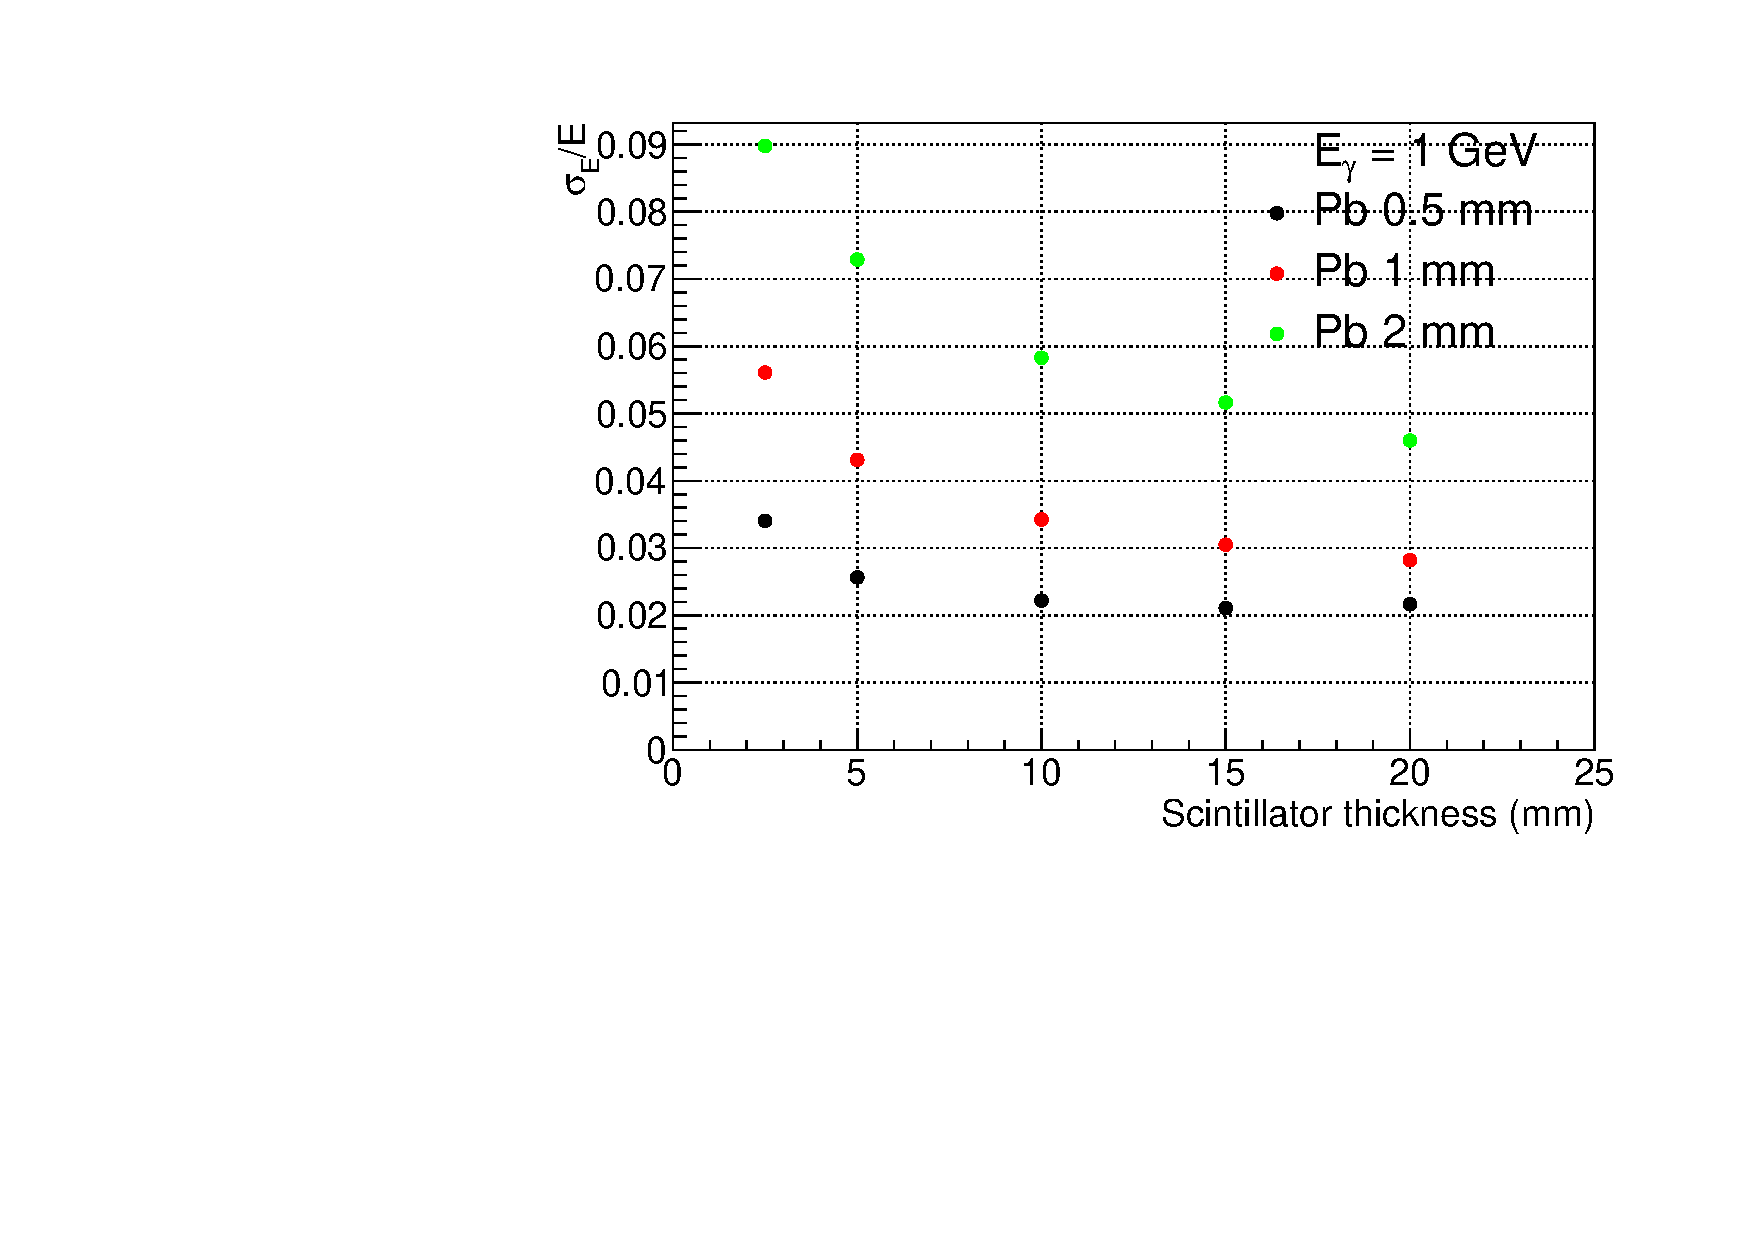
\includegraphics[width=0.48\textwidth]{figures/3.2/eres_thickness.pdf}
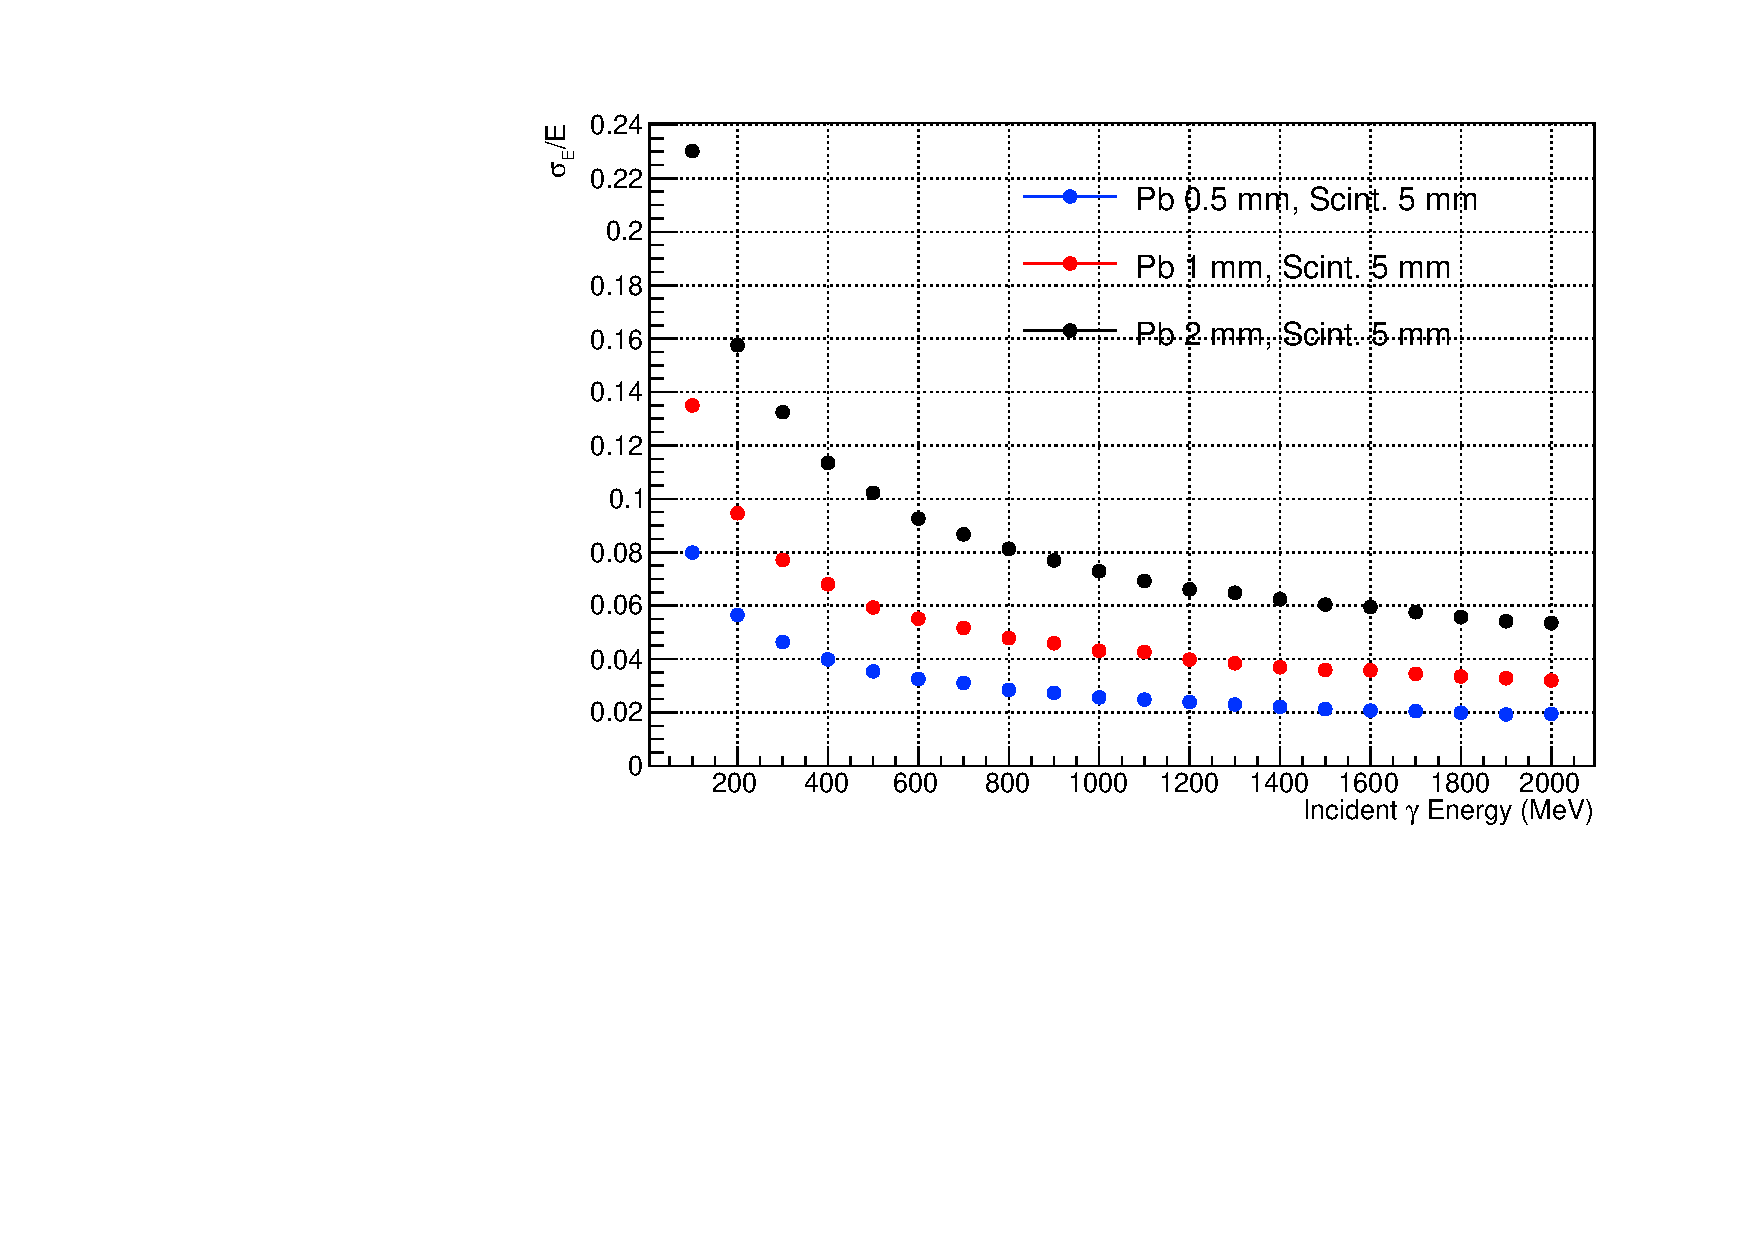
\includegraphics[width=0.48\textwidth]{figures/3.2/energy_resolution.pdf}
\caption{The dependence of the energy resolution on the thickness of scintillators(left) and the incident energy of $\gamma$(right)}
\label{fig:energy_res}
\end{figure}





%\subsection{Machine learning configuration}
%The configuration of the $\XGB$ can be organized with five parameters, described in Tab.~\ref{tab:XgbPar}. The parameters are selected as one providing better angular resolution. It is found that the Max. depth mostly affects the angular resolution, and the resolution is not enhanced for Max. depth~$>$~15 any more. It is also worth mentioning that configurations with N\_estimators larger than 1000 do not provide better resolution with the Max. depth~=~15. The angular resolution of the reconstruction is defined as the standard deviation of Gaussian function, whose parameters are evaluated by fitting the reconstructed angle distribution. Figure~\ref{fig:angle_reco_def} shows the reconstructed $\theta$ distribution with respect to each incident $\theta$ with described training parameters. The angular resolution for all $\theta$ is estimated to be 1.3~degree.

%\begin{figure}[!hbt]
%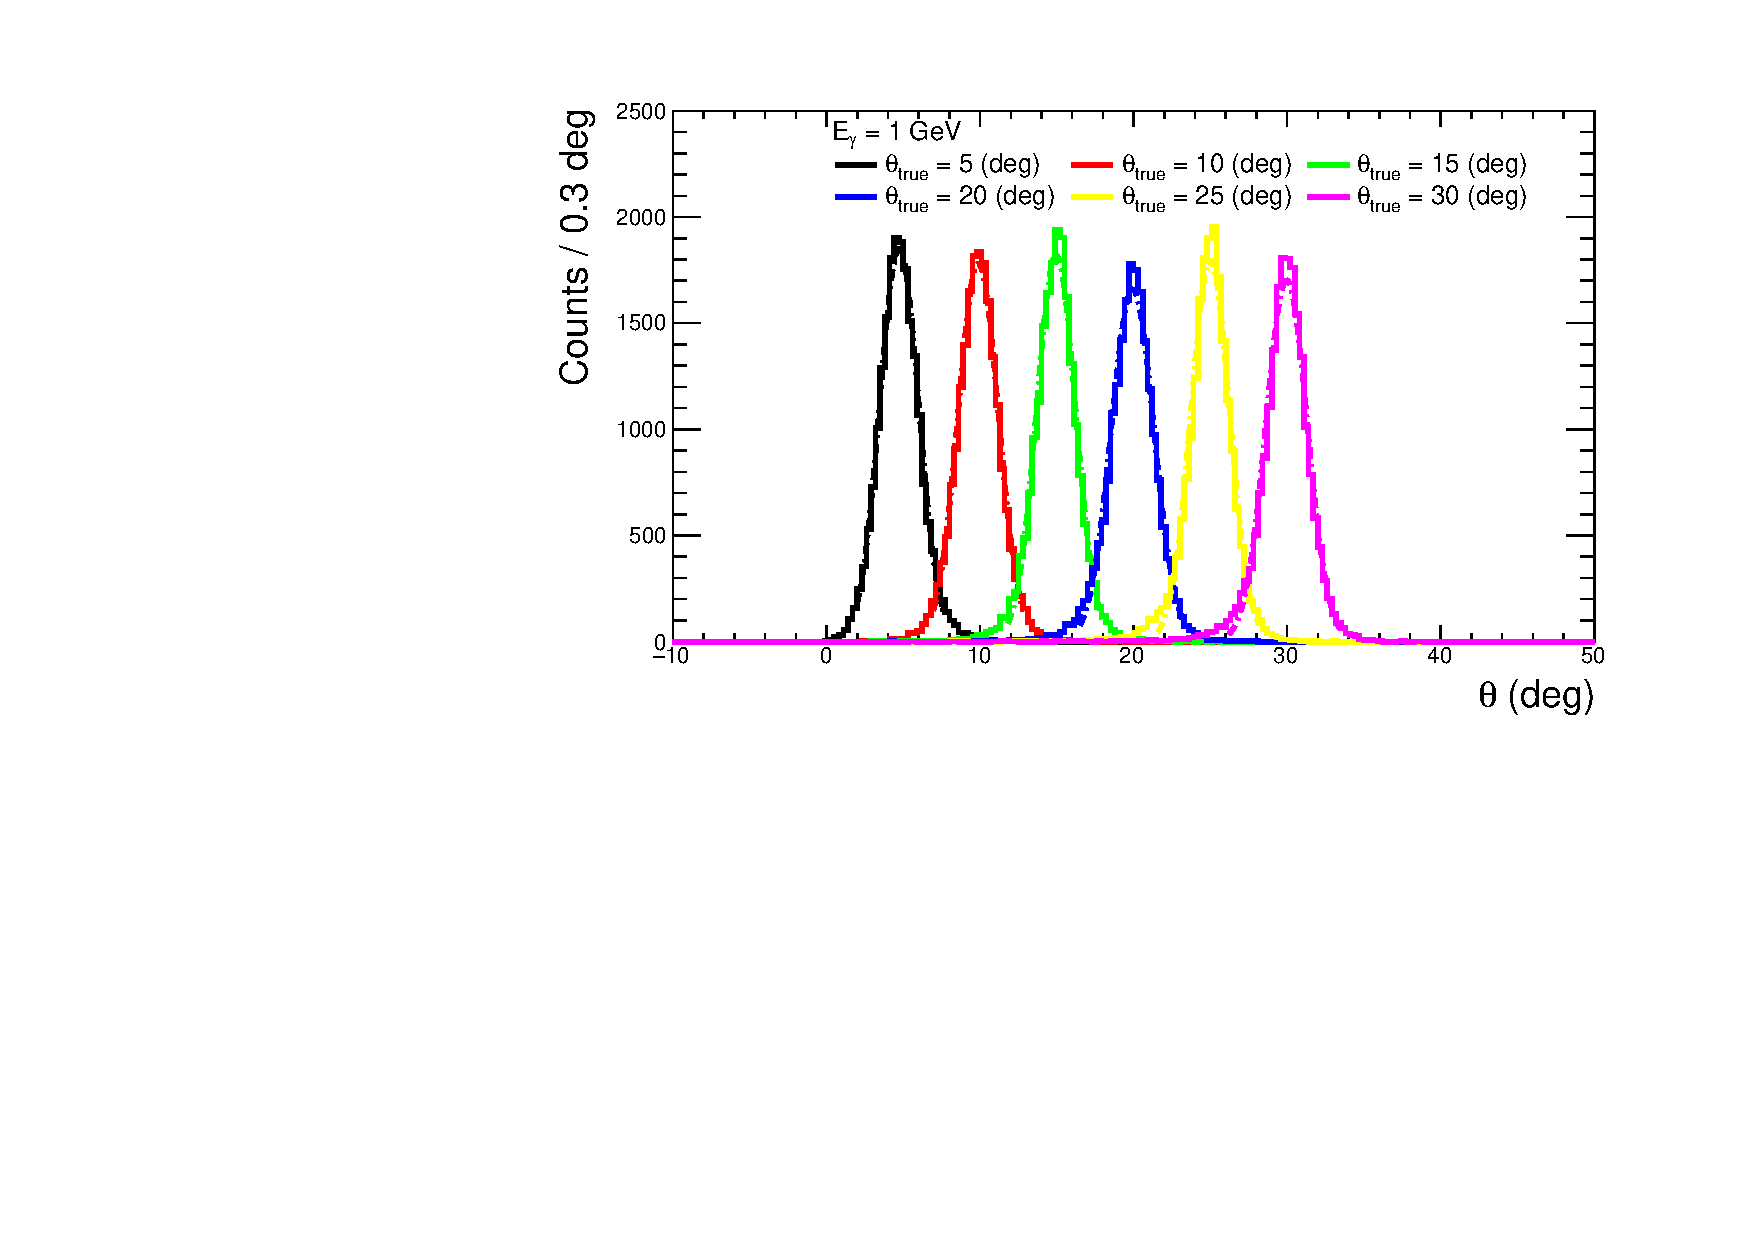
\includegraphics[width=0.89\textwidth]{figures/Fig1_reco_def.pdf}
%\caption{ (Color online) Reconstructed $\theta$ with respect to each true incident $\theta$ dotted lines denote each Gaussian function fitting the reconstructed $\theta$ distribution. The standard deviation of all Gaussian functions are estimated to be 1.3 degree.}
%\label{fig:angle_reco_def}
%\end{figure}

%\begin{table}[hbt!]
%\centering
%\caption{Parameterization of the $\XGB$}
%\begin{tabular}{cccc}
%\hline 
%Parameter & Function & Default value & Used value \\ \hline 
%N\_estimators & The number of decision trees & N.A. & 1000 \\  
%Max. depth & Possible maximum depth of tree structure & 6 & 15 \\ 
%Subsample & Fraction of total data used for a single decision & 1 & 1 \\ 
%Learning rate & Step length for calculation & 0.3 & 0.08 \\ 
%Gamma & Requirement on minimum loss function & 0 & 0 \\ 
%\hline
%\end{tabular}
%\label{tab:XgbPar}
%\end{table}

%\subsection{Detector dimension}
\subsection{Angle reconstruction using Machine Learning}

Figure~\ref{fig:angle_reco_def} shows the reconstructed $\theta$ obtained from the test samples, which are generated for fixed angles in range of $\theta=$ 5 to $\theta=$ 30 in 5 degrees steps. The number of generated gammas is $10^5$ and their energy is 1 GeV. The $\XGB$ correctly reconstructs $\theta=$ with a typical resolution as 1.2 degrees. There is no significant difference according to the incident angle. 

\begin{figure}[!hbt]
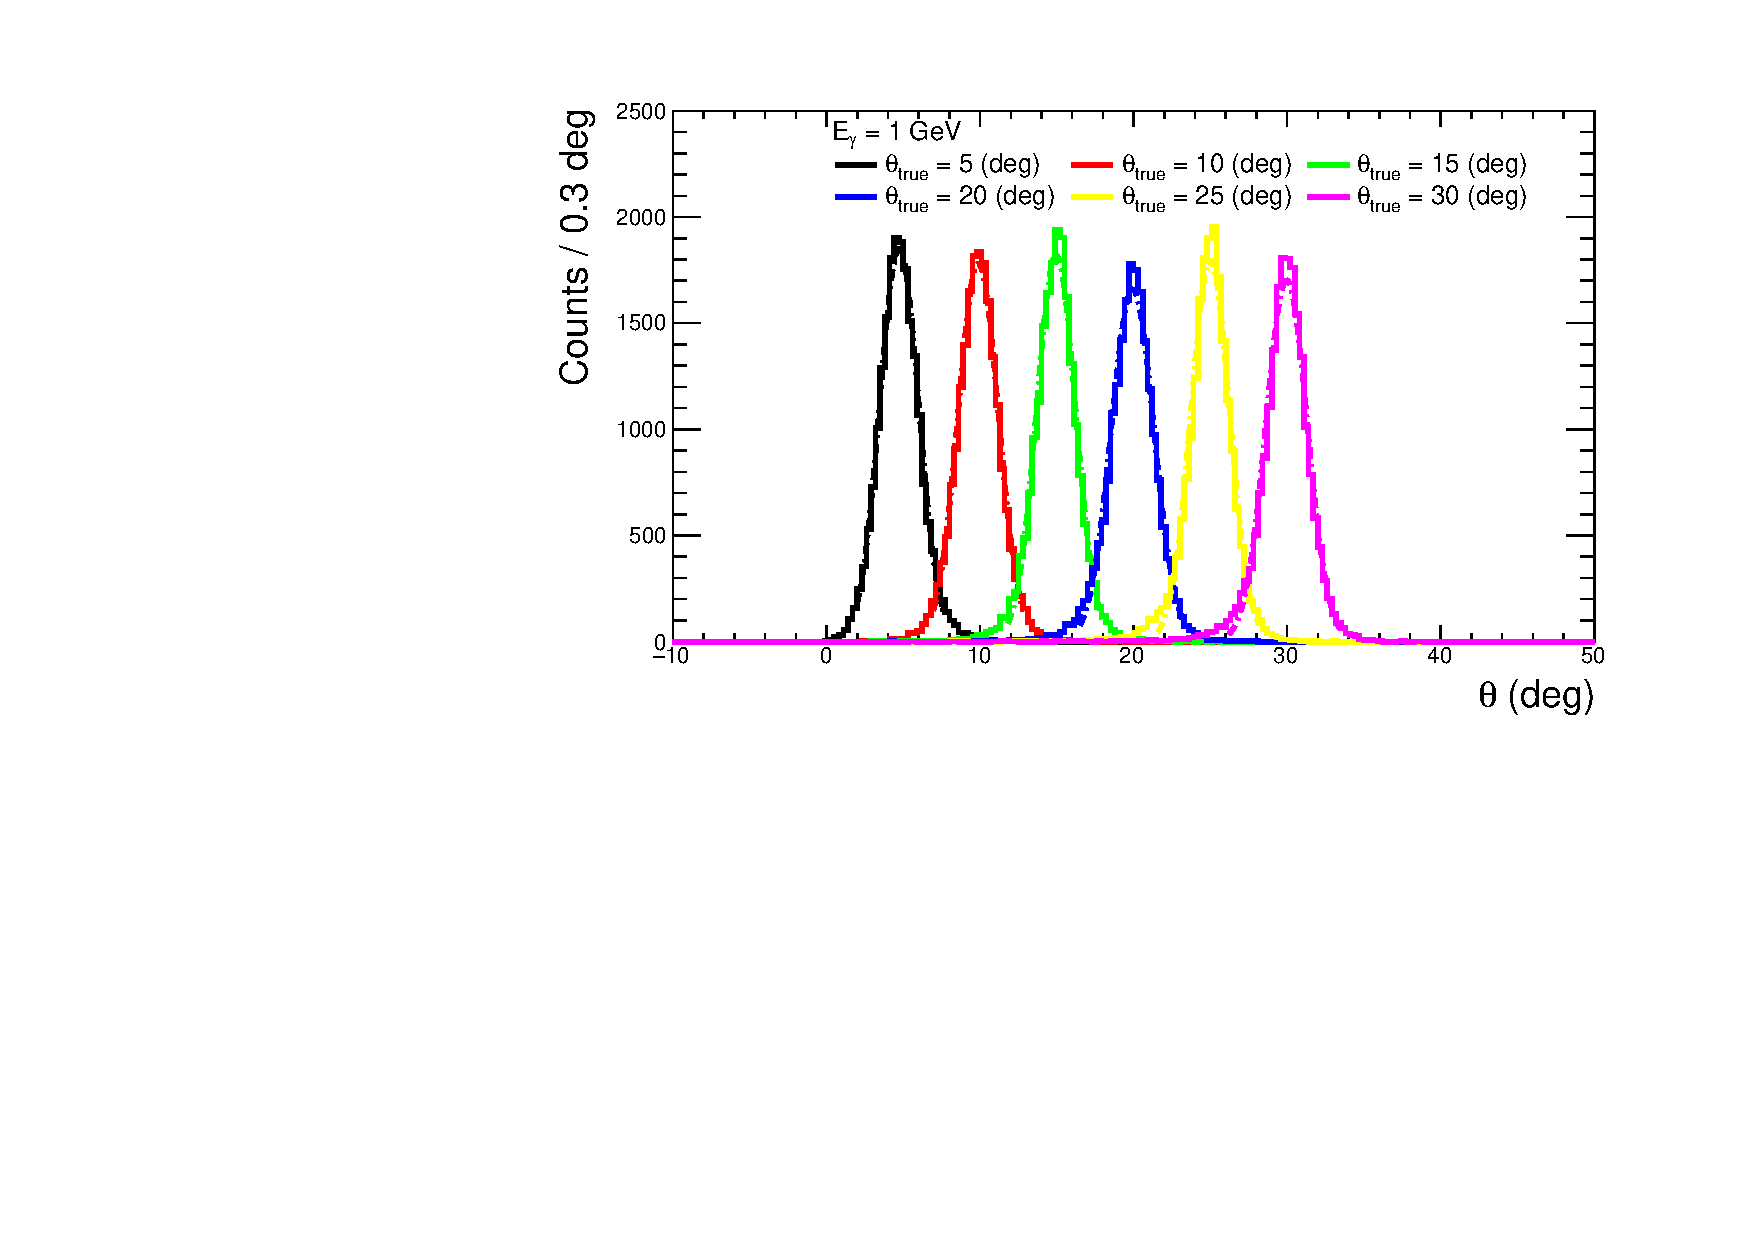
\includegraphics[width=0.89\textwidth]{figures/Fig1_reco_def.pdf}
\caption{ (Color online) Reconstructed $\theta$ with respect to each true incident $\theta$ dotted lines denote each Gaussian function fitting the reconstructed $\theta$ distribution. The standard deviation of all Gaussian functions are estimated to be 1.3 degree.}
\label{fig:angle_reco_def}
\end{figure}


\begin{figure}[!hbt]
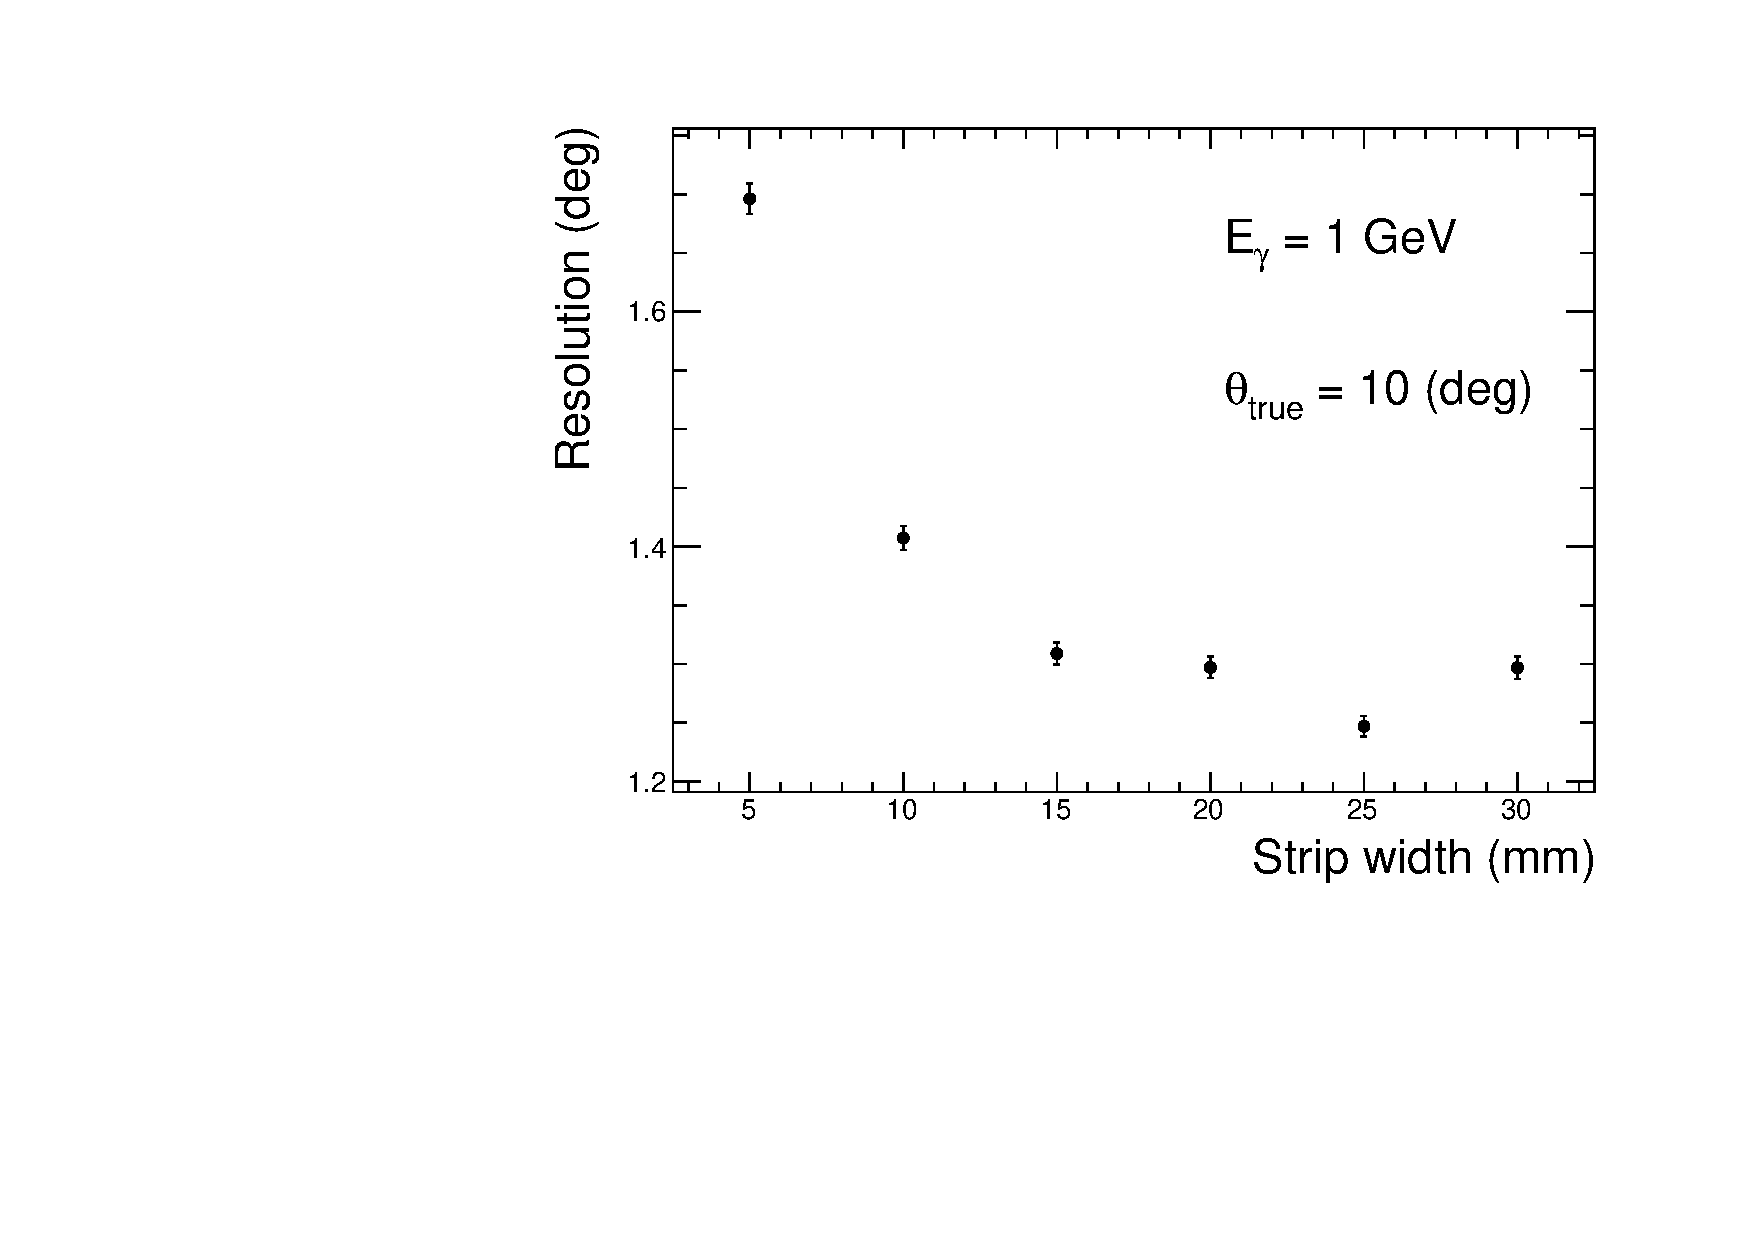
\includegraphics[width=0.58\textwidth]{figures/Fig2_reco_Width_width.pdf}
\caption{ The angular resolution as a function of the scintillator strip width for 1 GeV $\gamma$. The incident angle for each simulation is fixed as 10 degree.  }
\label{fig:angle_reco_width}
\end{figure}

With the narrower width of the scintillator strips, we may get more precise information about the shower shape. In order to find detector configuration providing the best angular resolution, we produced gamma events with changing the width of strips from 5 mm to 35 mm in 5 mm steps. As shown in Fig.~\ref{fig:angle_reco_width}, the narrower width doesn't give the better angular resolution. The main reason seems to be a limitation of the number of training sample caused by lack of computer memory.  As shown in Fig XXX, the obtained angular resolution for the 5-mm width becomes better with increasing the number of training sample, while the other larger width is saturated already. %achine learning for increasing number of input data. XXXX. 
Also, the angular resolution is not changed up to 25 mm in width of the strips, which means the more precise information is not essential for the better angular resolution because the shower generation is a stochastic process and low energy photons produced by the Compton scattering and photoelectric effects does not align the incident direction. 

%On the other hand, the finite size of the strip is related to the effect of incident gamma position. The previous results given in the Fig.~\ref{fig:angle_reco_width} are obtained from the data samples in which the incident gammas enter to a fixed position, the center of the strip. When we generated the gammas entering uniformly to the strip, we get the angular resolution as shown in Fig. xxx. Base on the results, we decide the width of the strip as xxx mm for a testing module to confirm the M.C. studies.
%The performance of the detector is tested with different detector dimensions. Different geometries are simulated in the Geant4 package and corresponding training procedures are applied with the same number of training events as 100,000. Figure~\ref{fig:angle_reco_width} shows the angular resolution of the reconstruction as a function of the scintillator strip width with 5-mm-wide steps. It if found that the configuration with 15-mm-wide strips provides better resolution than one with smaller strip widths, and configurations with larger strip size than 15 mm do not provide improved resolution so that the width of the strip is determined to be 15 mm.

\begin{figure}[!hbt]
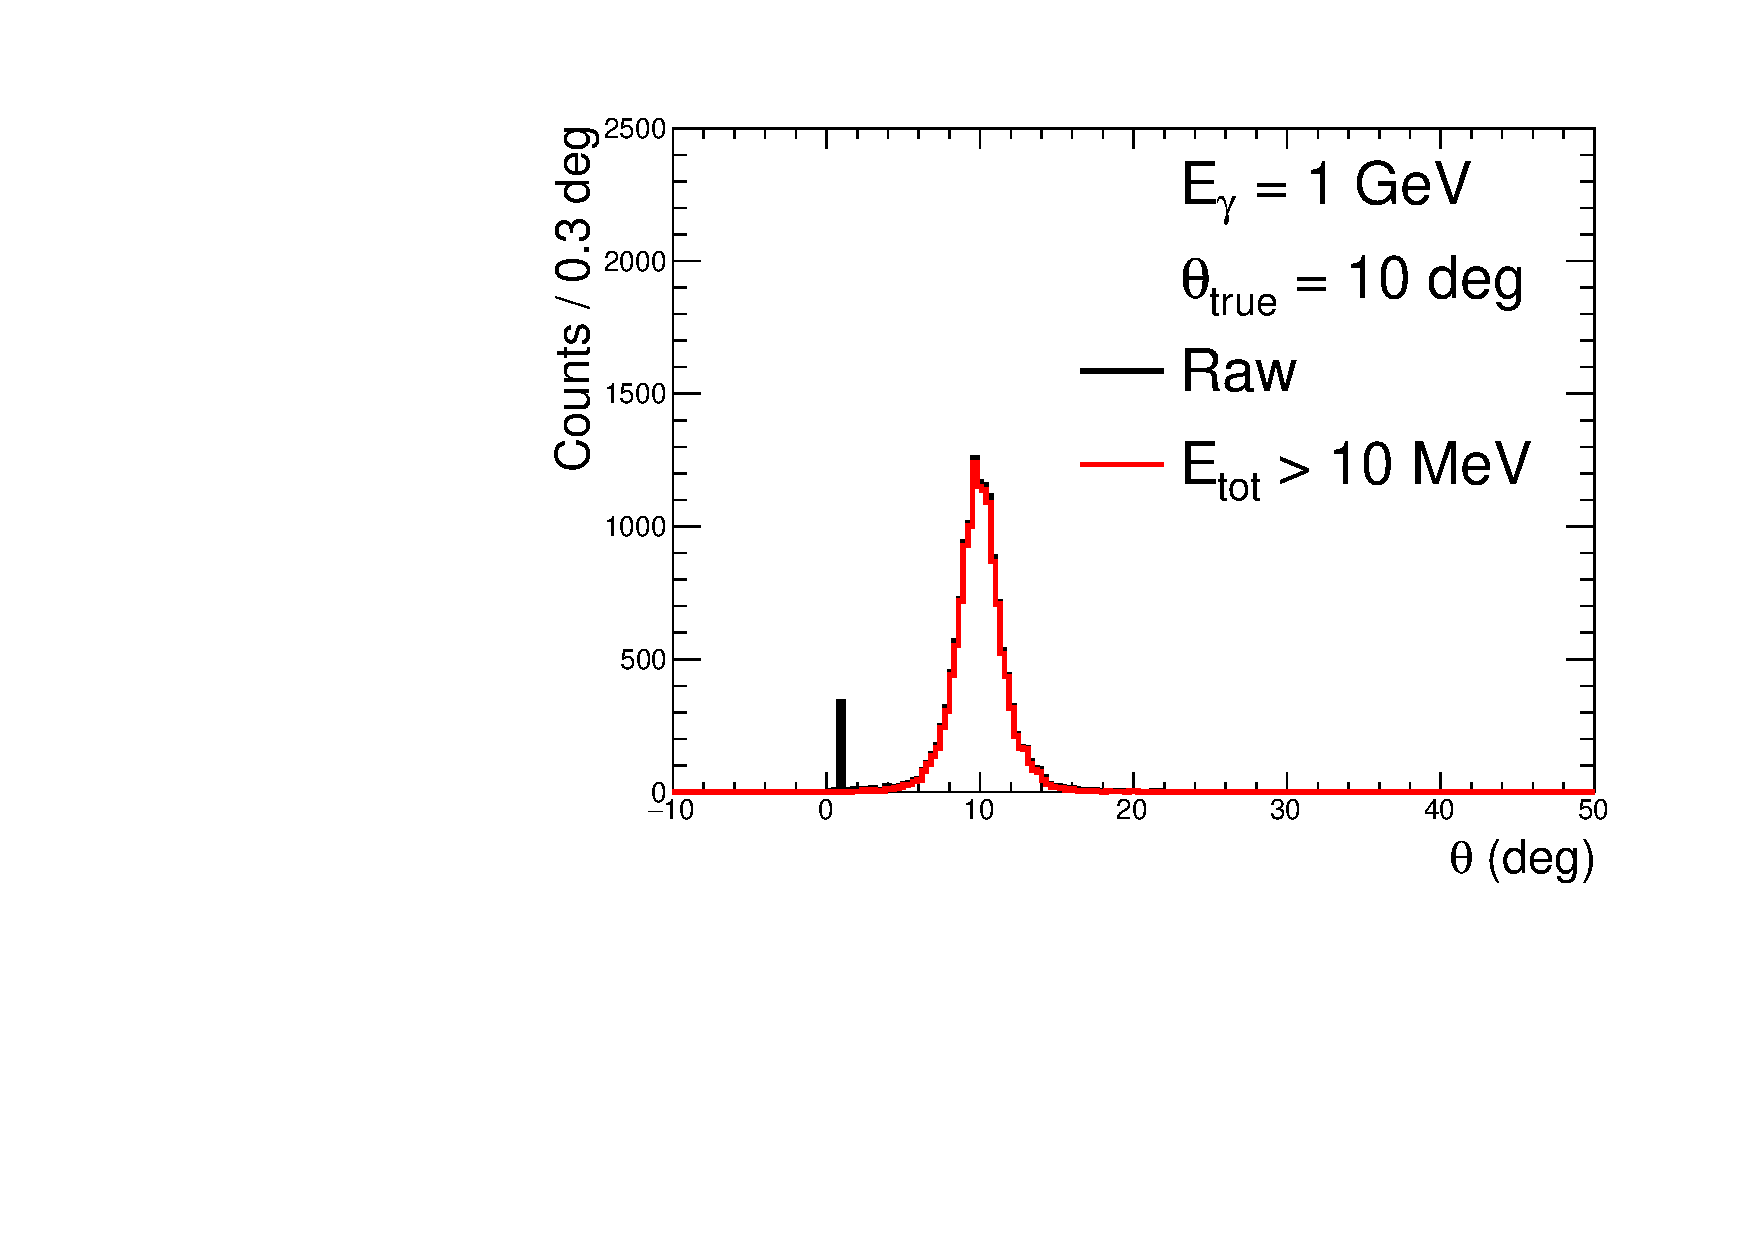
\includegraphics[width=0.48\textwidth]{figures/Fig3_reco_layer_hist.pdf}
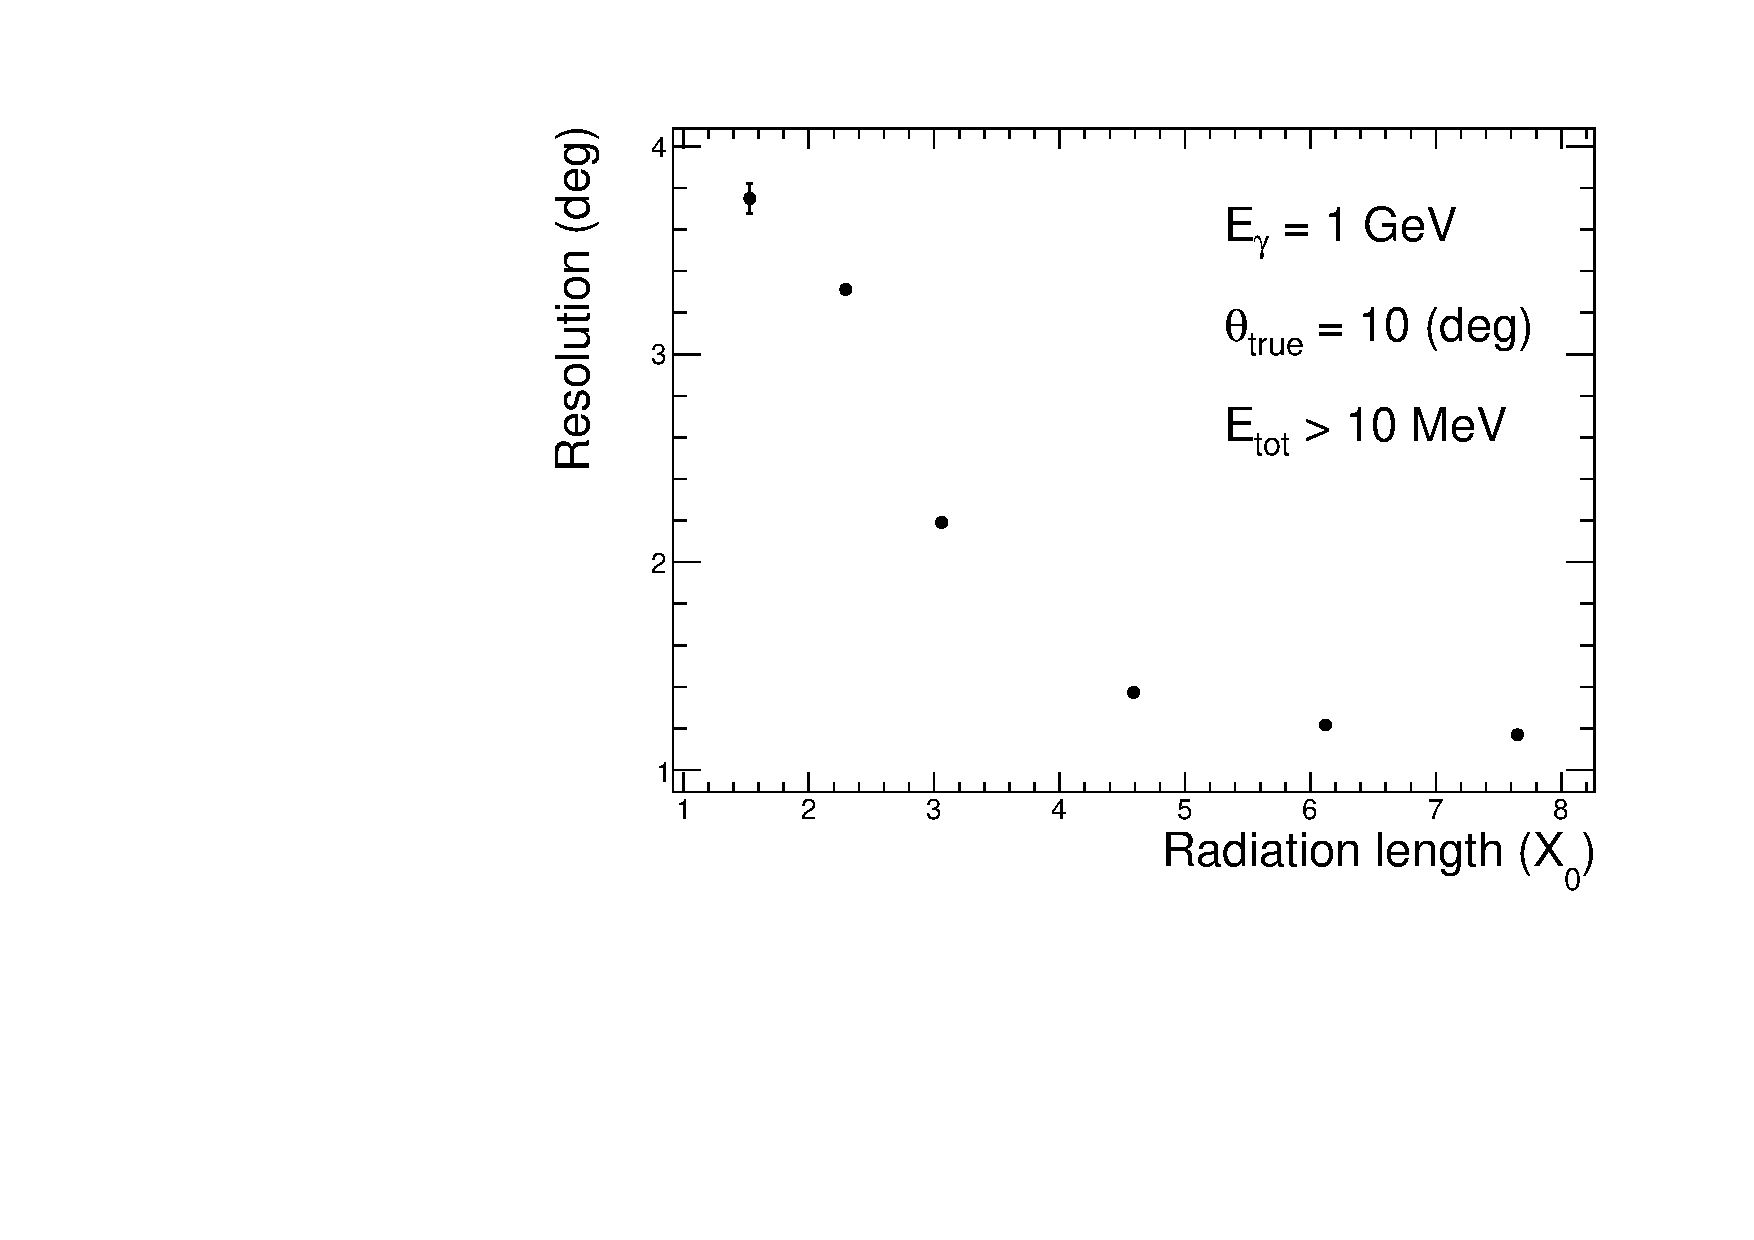
\includegraphics[width=0.48\textwidth]{figures/Fig3_reco_layer_graph.pdf}
\caption{ (Color online) Reconstructed $\theta$ for 1 GeV and $\theta_{\rm{true}}=$~10~deg $\gamma$ with (red) and without (black) the total energy ($E_{\rm{tot}}$) selection (left), and the angular resolution as a function of front layer depth used for the reconstruction (right). The inefficiency for 4.6$X_{0}$ is estimated to be 5.8\%  }
\label{fig:angle_reco_layer}
\end{figure}

When we focus only on the angle measurement, we don't need the full scale of the detector for containing the whole shower particles. We can reconstruct incident angle by using only the front-layer signals. % and check its performance.
%with the same configuration. 
As shown in Figure~\ref{fig:angle_reco_layer}, the angular resolution is not improved larger than 24 layers which corresponds to the 4.6$X_{0}$. With the energy threshold of 10 MeV to the first 24 layers, 94$\%$ of incident gammas are reconstructed correctly, and the remained 6$\%$ do not generate enough shower particles.

%reconstruction with the first 24 layers, which corresponds to the 4.6$X_{0}$, provides the identical resolution with one with the full geometry. The inefficiency can arise mainly due to no responses in the front region, and can be evaluated by comparing the number of events with and without applying the minimum total energy ($E_{\rm{tot}}$) threshold in the front region. The inefficiency for 4.6$X_{0}$ is estimated to be 5.8\%. Figure~\ref{fig:angle_reco_layer} shows the reconstructed $\theta$ distribution (left) and the angular resolution as a function of front layer depth used for the reconstruction (right). The reconstructed $\theta$ distribution without the $E_{\rm{tot}}$ threshold exhibits a delta peak near $\theta=$~0 as a results of failures of the $\theta$ reconstruction, and this peak clearly disappears by applying the $E_{\rm{tot}}$ threshold. The angular resolution is evaluated after applying the $E_{\rm{tot}}$ threshold, and estimated to be 1.3 deg, which is comparable results with fig.~\ref{fig:angle_reco_width} for 4.6$X_{0}$ depth, so that the radiation length for the $\theta$ reconstruction is determined to be 4.6$X_{0}$.

%The angle reconstruction is tested only with signals in front layers. Usages of front-layer signals are applied to the data sample for training and test procedures at the same time. The reconstruction with 24 layers, which possess 4.6$X_{0}$, provides the identical resolution with one with the full geometry. The inefficiency can arise mainly due to no responses in the front region, and can be evaluated by comparing the number of events with and without applying the minimum total energy ($E_{\rm{tot}}$) threshold in the front region. The inefficiency for 4.6$X_{0}$ is estimated to be 5.8\%. Figure~\ref{fig:angle_reco_layer} shows the reconstructed $\theta$ distribution (left) and the angular resolution as a function of front layer depth used for the reconstruction (right). The reconstructed $\theta$ distribution without the $E_{\rm{tot}}$ threshold exhibits a delta peak near $\theta=$~0 as a results of failures of the $\theta$ reconstruction, and this peak clearly disappears by applying the $E_{\rm{tot}}$ threshold. The angular resolution is evaluated after applying the $E_{\rm{tot}}$ threshold, and estimated to be 1.3 deg, which is comparable results with fig.~\ref{fig:angle_reco_width} for 4.6$X_{0}$ depth, so that the radiation length for the $\theta$ reconstruction is determined to be 4.6$X_{0}$.

%\begin{figure}[!hbt]
%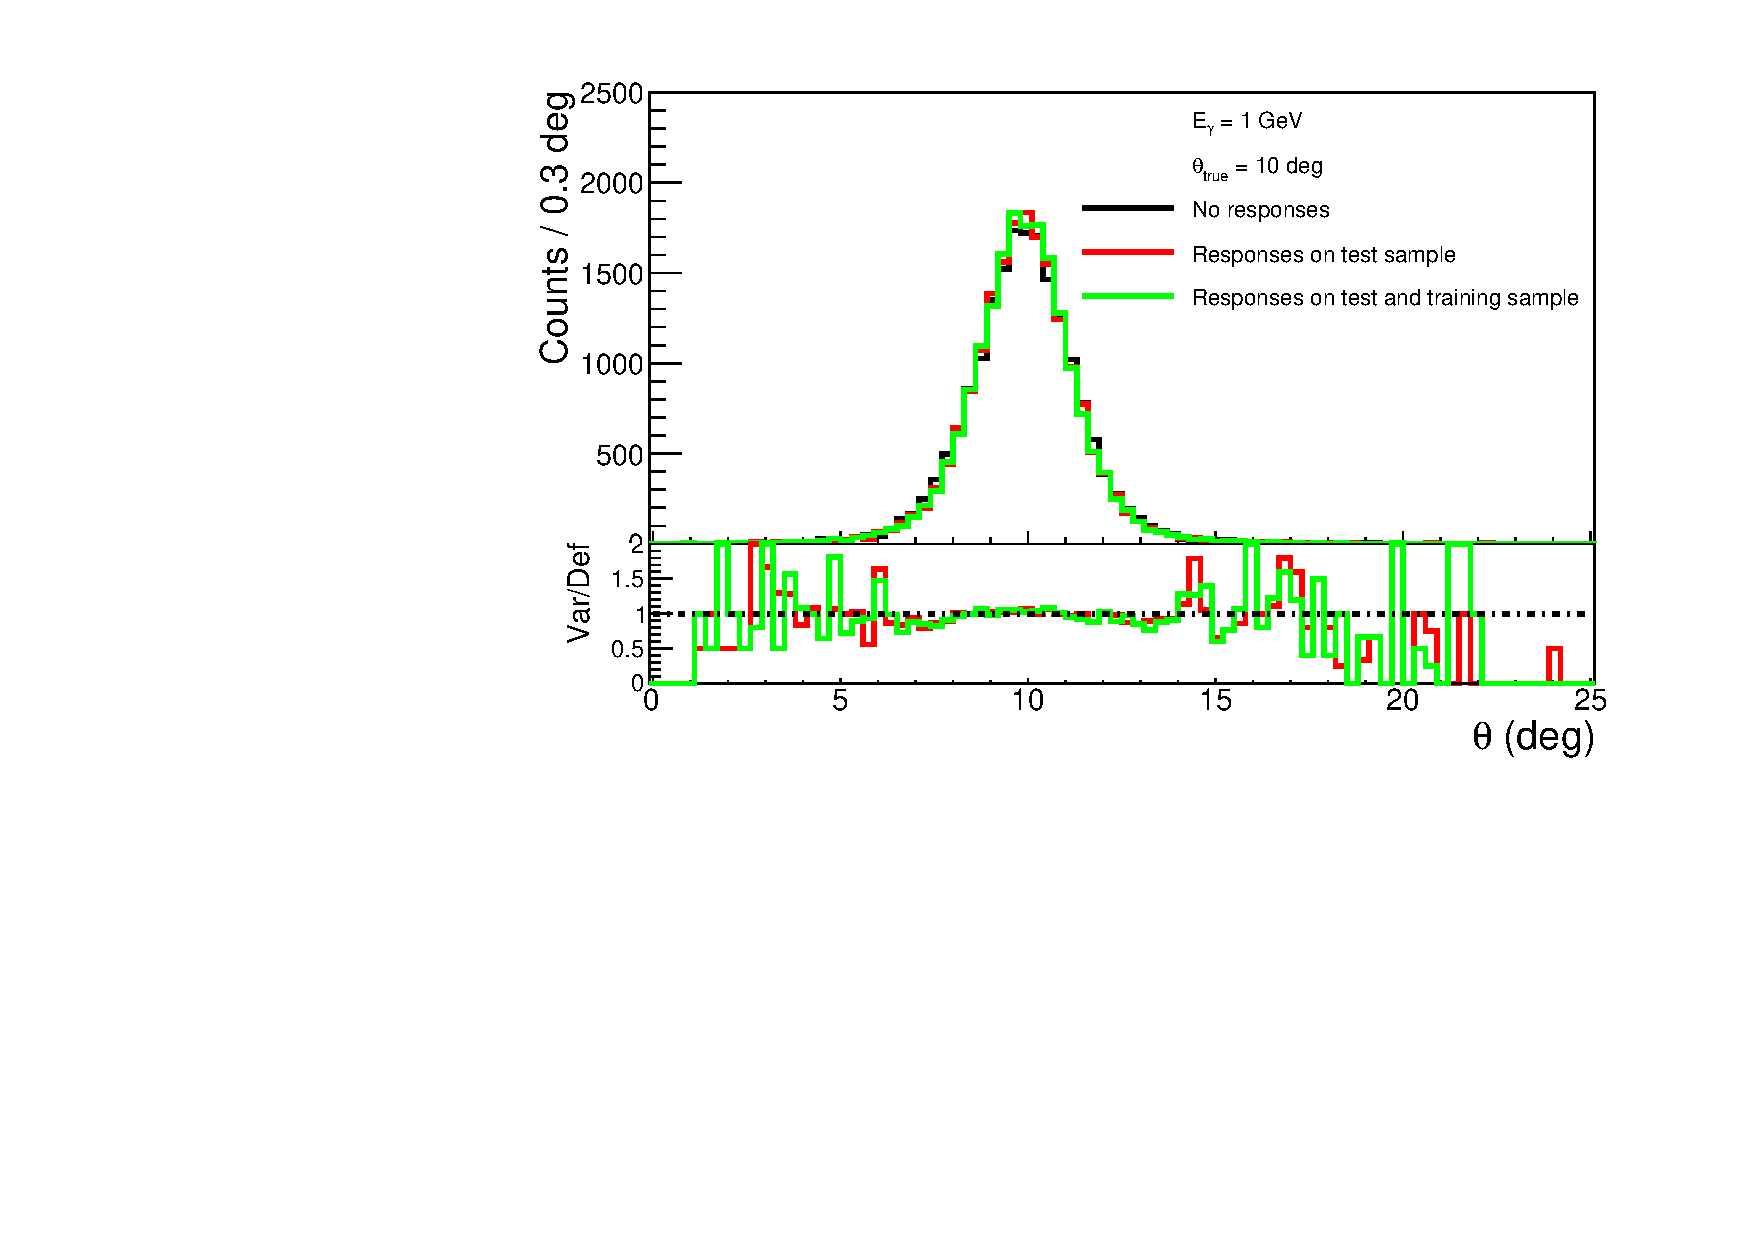
\includegraphics[width=0.8\textwidth]{figures/Fig4_reco_ecut.pdf}
%\caption{ (Color online) Reconstructed $\theta$ before (black) and after (red and green) applying the responses related with the energy measurement. The red (green) distribution is constructed with the training samples without (with) such effects and the test samples with such effects. Simulated effects are found to be not significant.}
%\label{fig:angle_reco_ecut}
%\end{figure}

- Threshold effect 

%\subsection{Expected performance}

%- W-Fiber 

%- Attenuation effect (NIM A715, pp48-55 (2013))

%- Light Yield (40/1mm $\rightarrow$ 200/MeV (UCV) other reference ?)


%The detector responses on the energy deposit are studied. The attenuation effect, smearing effect due to the photon statistics, and energy threshold for each channel are considered. The attenuation effect is applied to the deposit energy in each channel with the attenuation function, described in~\cite{Murayama:2020mcp}. The coefficients for the attenuation effect are assumed to be same with~\cite{Murayama:2020mcp}. The energy deposit after the attenuation effect is smeared with respect to the number of photon statistics. The number of photons ($\rm{n.p.e}$) is assumed to be 50 for 1 MeV. The standard deviation ($\sigma(E)$) for the smearing can be defined as 

%\begin{eqnarray}
%\sigma(E) = \sqrt{E/\rm{n.p.e}}
%\end{eqnarray}
%After the smearing attenuated energy deposit, the energy threshold (0.5 MeV) is applied to the all channels. These effects are applied to the test samples and the training samples, and the training is done with and without applying such effects and the test is done with applying the effects. Figure~\ref{fig:angle_reco_ecut} shows that the angular resolution is found to be not significant against such effects.

%\begin{figure}[!hbt]
%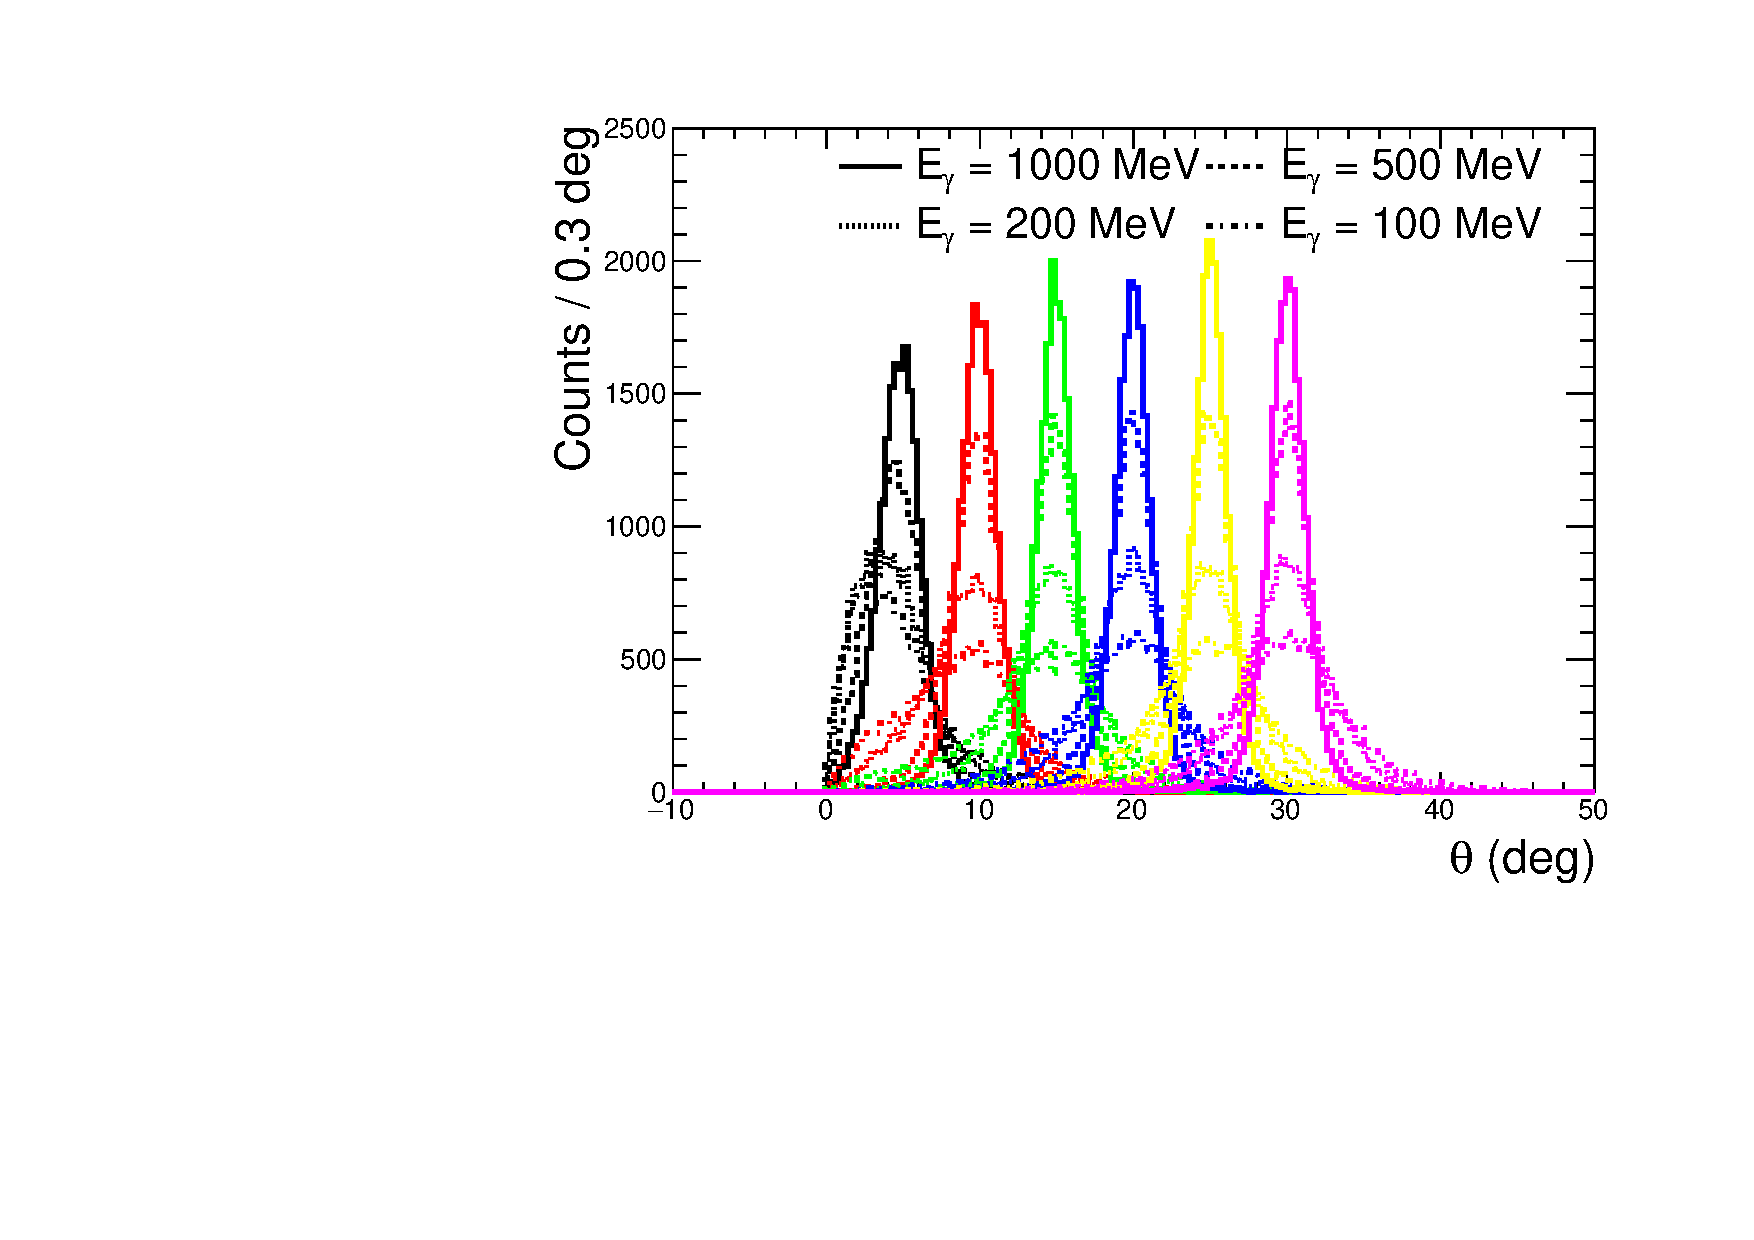
\includegraphics[width=0.6\textwidth]{figures/Fig5_reco_hist.pdf}
%\caption{ (Color online) Reconstructed $\theta$ with respect to each true incident $\theta$ and true %$\gamma$ energy. The incident $\theta_{\rm{true}}$ is illustrated with different colors, which are explained in fig.\ref{fig:angle_reco_def}, and the $\gamma$ energy is illustrated with different lines.}
%\label{fig:angle_reco_dep}
%\end{figure}

%The $\theta$ reconstruction dependencies on the incident angle and the incident energy are studied. Figure~\ref{fig:angle_reco_dep} shows the reconstructed $\theta$ with respect to the incident angle and the incident energy with different line colors and styles. The incident angle dependence of the reconstruction is found to be not significant for higher $E_{\gamma}>$~500~MeV and appears at lower $E_{\gamma}=$~200~MeV. The dependence on the incident energy can be clearly seen for all $\theta_{\rm{true}}$. The reconstruction for $\theta_{\rm{true}}=$~5~deg with lower $E_{\gamma}<$~200~MeV has a shifted maximum point due to their large standard deviations.


\begin{figure}[!hbt]
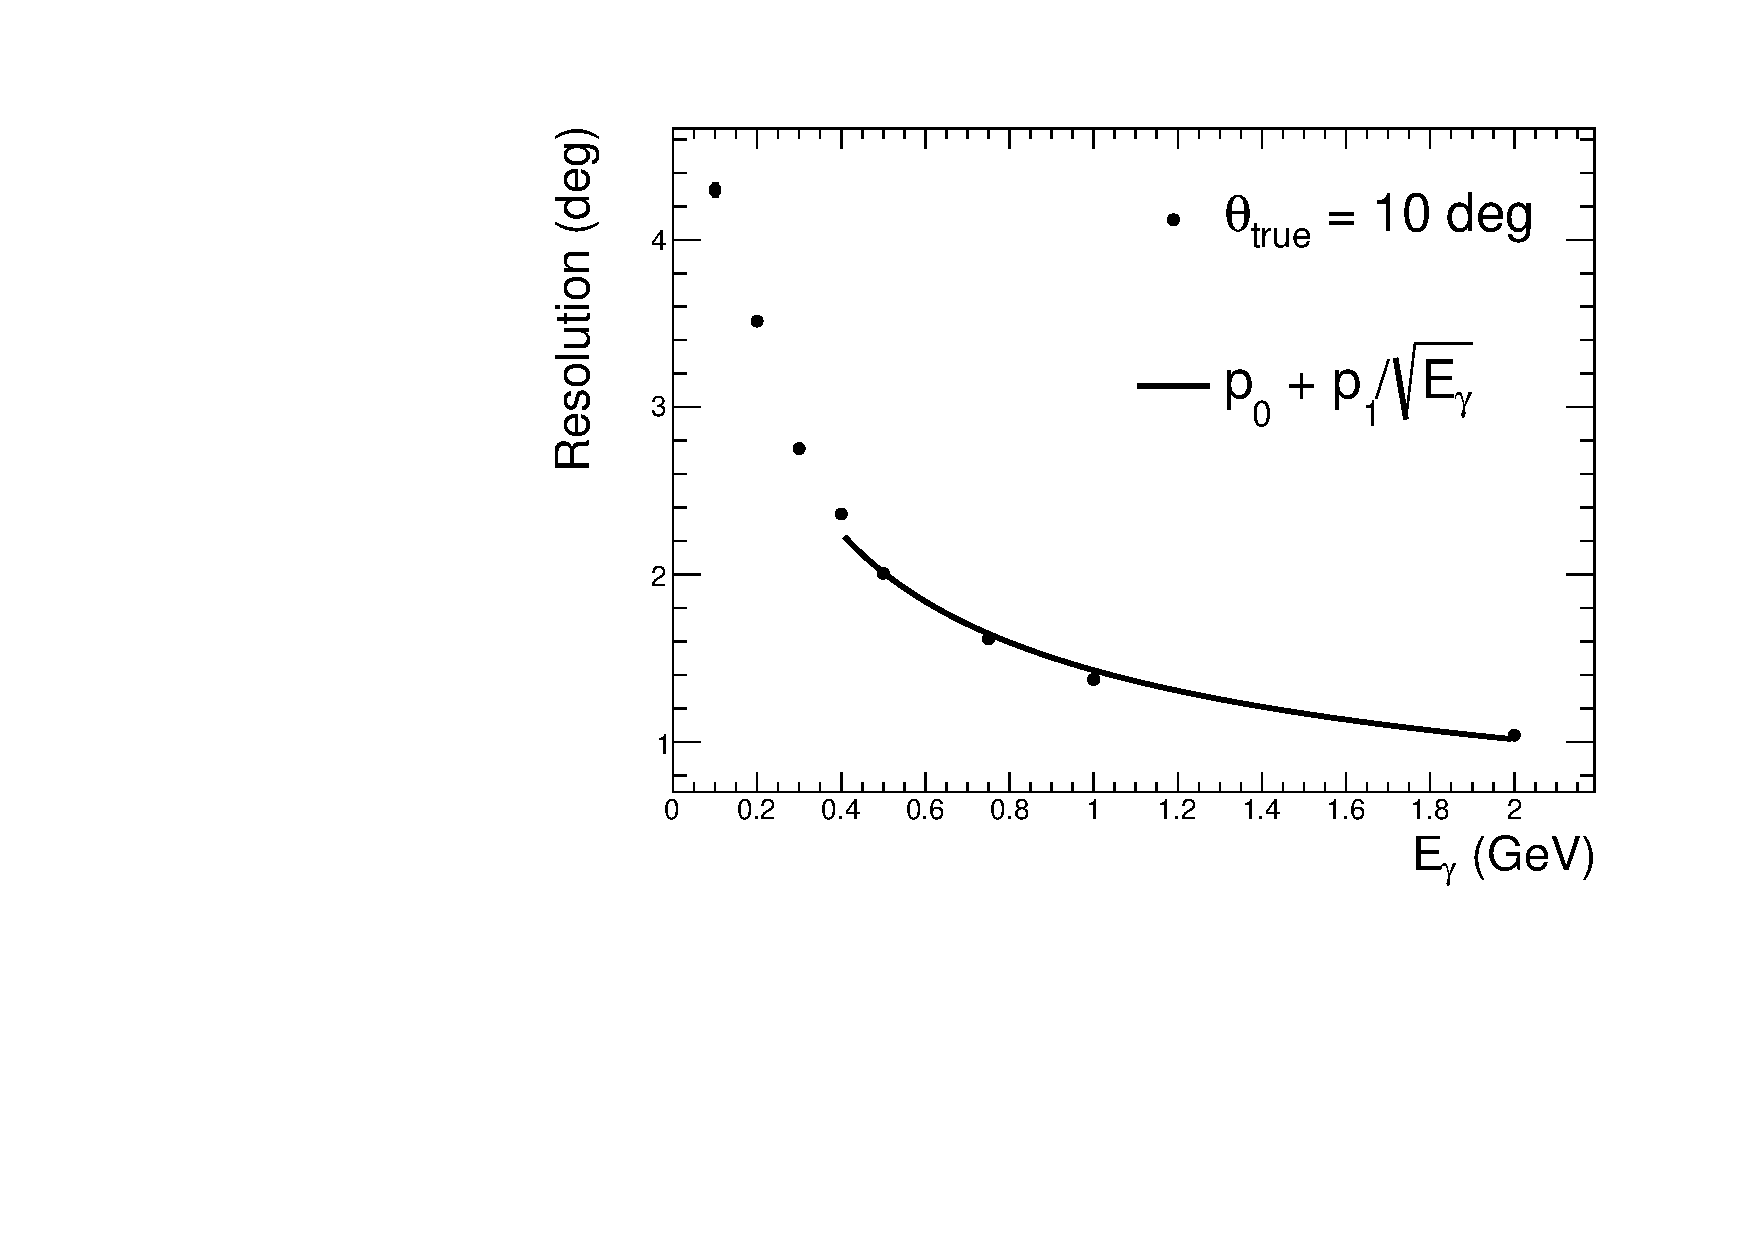
\includegraphics[width=0.48\textwidth]{figures/Fig5_reco_graph.pdf}
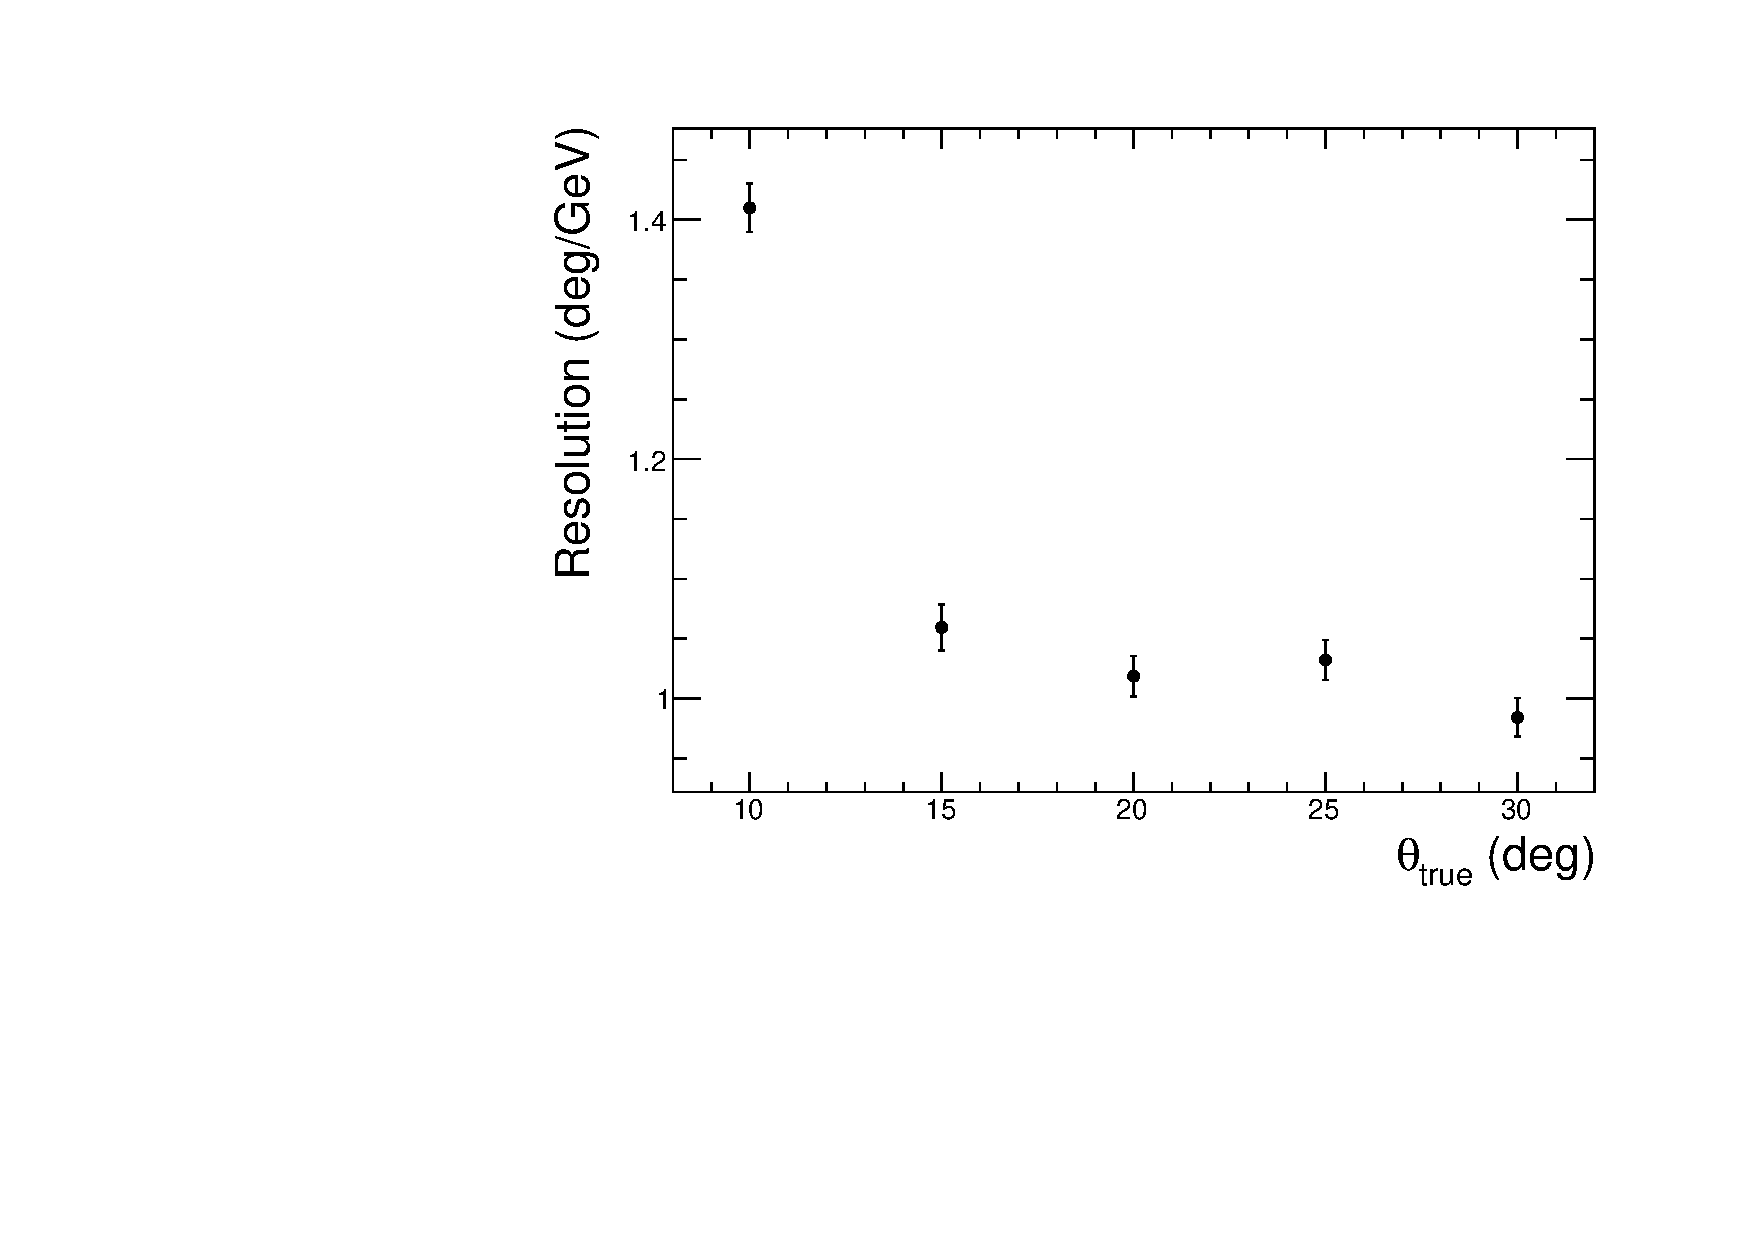
\includegraphics[width=0.48\textwidth]{figures/Fig5_reco_inc.pdf}
\caption{ The angular resolution as a function of $\gamma$ energy (left), and the angular resolution for 1 GeV as a function of incident $\theta_{\rm{true}}$ (right). }
\label{fig:angle_reco_dep_gr}
\end{figure}

Figure~\ref{fig:angle_reco_dep_gr} shows the angular resolution as a function of the incident $\gamma$ energy for $\theta_{\rm{true}}=$~10~deg on the left panel. The resolution is fitted with $p_{0} + p_{1}/\sqrt{E_{\gamma}}$, where the $p_{0}$ denotes the contribution from energy-independent term and is estimated to be zero, and the $p_{1}$ denotes the contribution from energy-dependent term, mainly related with the development of the EM shower. The estimated $p_{1}$ for different $\theta_{\rm{true}}$ can be seen in the right panel of fig.~\ref{fig:angle_reco_dep_gr}. They are deviating within $\pm$~0.05~deg range from the 1.25~deg.

\section{Conclusions}
We studied the sampling calorimeter to measure incident angle of the gamma. With the configuration of alternation 1-mm thick lead sheets and 5-mm thick plastic scintillators will produce the energy resolution as 4$\%$  for 1 GeV gamma due to the sampling fluctuation. When we focus only on the angle measurement, the first 24 layers (4.6 Xo) produce the same resolution as that of the full geometry (20 Xo) with 94$\%$ of detection efficiency. The angular resolution is not changed significantly increasing the width of the strips up to 25mm and expected to be 1.2 degrees for the 1 GeV gamma.

https://github.com/chenkkkk/MTR-TSF

\label{sec:con}


%\pagebreak

\begin{acknowledgments}
\end{acknowledgments}

\bibliography{paper}

\end{document}
